\documentclass[GTS.tex]{subfiles}
%\usepackage{amsmath,amssymb}
%\usepackage[utf8]{inputenc}
%\usepackage[spanish]{babel}
%\usepackage[]{graphicx}
%\usepackage{enumerate}
%\usepackage{amsthm}
%\usepackage{tikz-cd}
%\usetikzlibrary{babel}
%\usepackage{pgf,tikz}
%\usepackage{mathrsfs}
%\usetikzlibrary{arrows}
%\usetikzlibrary{cd}
%\usepackage[spanish]{babel}
%\usepackage{fancyhdr}
%\usepackage{titlesec}
%\usepackage{floatrow}
%\usepackage{makeidx}
%\usepackage[tocflat]{tocstyle}
%\usetocstyle{standard}
%\usepackage{svg}
%\usepackage{epstopdf}
%%\usepackage[sc]{mathpazo}
%%\usepackage{blindtext}
%\usepackage{color}   %May be necessary if you want to color links
%\usepackage{hyperref}
%\hypersetup{colorlinks=true,citecolor=red, linkcolor=blue}
%
%
%\renewcommand{\baselinestretch}{1,4}
%\setlength{\oddsidemargin}{0.25in}
%\setlength{\evensidemargin}{0.25in}
%\setlength{\textwidth}{6in}
%\setlength{\topmargin}{0.1in}
%\setlength{\headheight}{0.1in}
%\setlength{\headsep}{0.1in}
%\setlength{\textheight}{8in}
%\setlength{\footskip}{0.75in}
%
%\newtheorem{teorema}{Teorema}[section]
%\newtheorem{defi}[teorema]{Definición}
%\newtheorem{coro}[teorema]{Corolario}
%\newtheorem{lemma}[teorema]{Lema}
%\newtheorem{ej}[teorema]{Ejemplo}
%\newtheorem{ejs}[teorema]{Ejemplos}
%\newtheorem{observacion}[teorema]{Observación}
%\newtheorem{observaciones}[teorema]{Observaciones}
%\newtheorem{prop}[teorema]{Proposición}
%\newtheorem{propi}[teorema]{Propiedades}
%\newtheorem{nota}[teorema]{Nota}
%\newtheorem{notas}[teorema]{Notas}
%\newtheorem*{dem}{Demostración}
%\newtheorem{ejer}[teorema]{Ejercicio}
%\newtheorem{consec}[teorema]{Consecuencia}
%\newtheorem{consecs}[teorema]{Consecuencias}
%
%\providecommand{\abs}[1]{\lvert#1\rvert}
%\providecommand{\norm}[1]{\lVert#1\rVert}
%\providecommand{\ninf}[1]{\norm{#1}_\infty}
%\providecommand{\numn}[1]{\norm{#1}_1}
%\providecommand{\gabs}[1]{\left|{#1}\right|}
%\newcommand{\bor}[1]{\mathcal{B}(#1)}
%\newcommand{\R}{\mathbb{R}}
%\newcommand{\N}{\mathbb{N}}
%\newcommand{\Q}{\mathbb{Q}}
%\newcommand{\C}{\mathbb{C}}
%\newcommand{\Pro}{\mathbb{P}}
%\newcommand{\Tau}{\mathcal{T}}
%\newcommand{\verteq}{\rotatebox{90}{$\,=$}}
%\newcommand{\vertequiv}{\rotatebox{110}{$\,\equiv$}}
%\providecommand{\lrg}{\longrightarrow}
%\providecommand{\func}[2]{\colon{#1}\longrightarrow{#2}}
%\newcommand*{\QED}{\hfill\ensuremath{\blacksquare}}
%\newcommand*\circled[1]{\tikz[baseline=(char.base)]{
%            \node[shape=circle,draw,inner sep=1.5pt] (char) {#1};}}
%\newcommand*{\longhookarrow}{\ensuremath{\lhook\joinrel\relbar\joinrel\rightarrow}}
%
%\def\quot#1#2{%
%    \raise1ex\hbox{$#1$}\Big/\lower1ex\hbox{$#2$}%
%}
%
%\makeatletter
%\renewcommand\tableofcontents{%
%  \null\hfill\textbf{\Large\contentsname}\hfill\null\par
%  \@mkboth{\MakeUppercase\contentsname}{\MakeUppercase\contentsname}%
%  \@starttoc{toc}%
%}
%
%\pagestyle{fancy}
%\fancyhf{}
%\rhead{Topología de Superficies (Grado en Matemáticas)}
%\lhead{Curso 2016/2017}
%\cfoot{\thepage}

\begin{document}
%\title{Topología de Superficies}
%\author{Antonio Rafael Quintero Toscano\\ Javier Aguilar Martín}
%\date{Curso 2016/2017}
%\maketitle

\renewcommand\chaptername{\Huge Tema}

\titleformat{\chapter}[display]
    {\normalfont\huge\bfseries}{\chaptertitlename\ \thechapter}{10pt}{\Huge}
\titlespacing*{\chapter}{0pt}{-1cm}{10pt}

  

\setcounter{chapter}{1}

\chapter{Clasificación de Superficies I}
En topología, clasificar la familia de espacios que cumplen una propiedad topológica (es decir, invariante por homeomorfismos) $P$ consiste en alcanzar los siguientes objetivos:
\begin{enumerate}
\item[$\circled{1}$] Encontrar modelos $X_1,\dots,X_n,\dots$ de forma que todo espacio topológico con la propiedad $P$ es homeomorfo a algún $X_i$.
\item[$\circled{2}$] Dar un método de ``distinguibilidad", es decir, un procedimiento o técnica que distinga cuándo dos espacios $X$ e $Y$ con la propiedad $P$ \underline{no} son homemorfos. Para ello, bastará distinguir los modelos $X_i$.
\end{enumerate}
Algunas de las propiedades conocidas desde el curso de Topología de 1º son:
\begin{itemize}
\item Compacidad.
\item Conexión.
\item Número de componentes conexas (por caminos).
\item Número y orden de puntos de corte.
\end{itemize}


\section{Teorema de Clasificación de Superficies}

\begin{defi} Una \textbf{superficie sin borde} es un espacio topológico $X$ cumpliendo el axioma de separación $T_2$ y el segundo axioma de numerabilidad, tal que todo $x\in X$ posee un entorno homeomorfo a una bola abierta de $\R^2$ con la topología euclídea.
\end{defi}

\begin{defi} Una \textbf{superficie con borde} es un espacio topológico $X$ cumpliendo el axioma de separación $T_2$ y el segundo axioma de numerabilidad, tal que todo $x\in X$ posee un entorno homeomorfo a $\R^2_+$. Los puntos que poseen un entorno de este tipo pero no poseen uno homeomorfo $B^2$ forman la \textbf{frontera} de la superficie, denotada $\partial X$.
\end{defi}

\begin{teorema}[de inmersión de Whitney] Toda superficie $M$ admite una inmersión en $\R^4$. En particular, $M$ posee topología euclídea. 
\end{teorema}

\begin{nota} Este resultado es más general; para una variedad topológica (este concepto se verá en el próximo curso) de dimensión $m$ siempre existe una inmersión en $\R^{2m}$.
\end{nota}



Ya hemos visto que la esfera y el plano proyectivo tienen los siguientes modelos dados como espacios cociente.

\definecolor{qqqqff}{rgb}{0.3333333333333333,0.3333333333333333,0.3333333333333333}
\begin{tikzpicture}[line cap=round,line join=round,>=triangle 45,x=1.0cm,y=1.0cm]
\clip(-2.6533333333333338,-1.3) rectangle (12.68,2);
\draw [color=black,fill=qqqqff,fill opacity=0.1] (2.,0.) circle (1.cm);
%\fill[color=qqqqff,fill=qqqqff,fill opacity=0.01] (2.,0.) circle (1.cm);
\draw [color=black,fill=qqqqff, fill opacity=0.1] (6.,0.) circle (1.cm);

\draw [->] (1.9082829505087413,0.9957851087622359) -- (2.19363303189666,0.9810740282764124);
\draw [->] (1.880854779381569,-0.992876838486922) -- (2.1046847845180428,-0.994505452921406);
\draw [->] (5.900496280979001,0.9950371902099892) -- (6.099503719020999,0.9950371902099892);
\draw [->] (6.104684784518044,-0.9945054529214059) -- (5.895315215481959,-0.9945054529214061);
\draw (1.9,1.4) node[anchor=north west] {$a$};
\draw (1.9,-0.9466666666666669) node[anchor=north west] {$a$};
\draw (0.5,0.2666666666666667) node[anchor=north west] {$p$};
\draw (3,0.2533333333333334) node[anchor=north west] {$q$};
\draw (4.5,0.17333333333333337) node[anchor=north west] {$p$};
\draw (7.1,0.17333333333333337) node[anchor=north west] {$p$};
\draw (1,1.1) node[anchor=north west] {$x$};
\draw (1,-0.8) node[anchor=north west] {$x$};
\draw (2.853333333333334,0.9) node[anchor=north west] {$b$};
\draw (2.72,-0.5466666666666667) node[anchor=north west] {$b$};
\draw (0.44,1.6533333333333338) node[anchor=north west] {$S^2$};
\draw (4.546666666666668,1.626666666666667) node[anchor=north west] {$\mathbb{P}_2\mathbb{R}$};
\begin{scriptsize}
\draw [fill=black] (1.,0.) circle (2.5pt);
\draw [fill=black] (5.,0.) circle (2.5pt);
\draw [fill=black] (3.,0.) circle (2.5pt);
\draw [fill=black] (7.,0.) circle (2.5pt);
\draw [fill=black] (1.2928932188134525,0.7071067811865476) circle (1.5pt);
\draw [fill=black] (1.2928932188134525,-0.7071067811865476) circle (1.5pt);
\draw [fill=black] (2.7205717590143914,0.6933803718817729) circle (1.5pt);
\draw [fill=black] (2.713684088491497,-0.7004677164823951) circle (1.5pt);
\end{scriptsize}
\end{tikzpicture}

El siguiente teorema proporcionará modelos para todas las demás superficies.

\begin{teorema}
Una superficie compacta y conexa distinta de $S^2$ y $\Pro_2\R$ es homeomorfa a un espacio cociente de alguno de los siguientes tipos o a una suma conexa finita de ellos (esta operación se verá más adelante):
\begin{itemize}
\item \textbf{Tipo I ($M_n$)}
El resultado de identificar los lados de un polígono (llamado polígono fundamental) de $4n$ lados de acuerdo al código $a^{}_1 b^{}_1 a^{-1}_1 b^{-1}_1\dots\ a^{}_n b^{}_n a_n^{-1} b_n^{-1}$. A una superficie de este tipo se la llama \textbf{superficie orientable de género} $\mathbf{n}$. La esfera se considera orientable de género $0$.

Recordemos que esto significa que, fijado un sentido de giro sobre el polígono, las aristas indicadas con la misma letra e índice deben identificarse de manera que, por ejemplo,  $a_i$ indica que los puntos de la arista van apareciendo en el sentido del giro, mientras que esos mismos puntos en  $a_i^{-1}$ se ven aparecer  en el sentido opuesto.

\definecolor{zzttqq}{rgb}{0.6,0.2,0.}
\begin{center}
\begin{tikzpicture}[line cap=round,line join=round,>=triangle 45,x=1.0cm,y=1.0cm]
\clip(-8.12,-0.5) rectangle (5.853333333333331,2);

\fill [color=zzttqq,fill=zzttqq, fill opacity=0.1] (-3.7733333333333365,1.2466666666666635) -- (-2.9733333333333367,1.26) -- (-1.9066666666666698,0.8066666666666639) -- (-2.56,0.) -- (-3.52,-0.12666666666666884) -- (-3.673611239467886,-0.13773171459531575) -- (-3.777057115666006,-0.12596930424422792) -- (-3.875606206429468,-0.0996531230038682) -- (-3.977353849189612,-0.05498092886738859) -- (-4.0760538038806,0.009380129353487532) -- (-4.162935951831398,0.08987067656754544) -- (-4.2341700903315225,0.18264700512963727) -- (-4.295422813458533,0.3017926849306371) -- (-4.329730043718338,0.41515532979662517) -- (-4.344917909096754,0.5608706321820421) -- (-4.326408918240099,0.7197060643226713) -- (-4.291819151924729,0.8270839312293088) -- (-4.217546842365534,0.9620589267129689) -- (-4.13464511731667,1.0594322649336707) -- (-4.050334781046338,1.1297434589257818) -- (-3.9721215332585897,1.177765882326943) -- (-3.8785344542937956,1.218629550366861) -- cycle;
\fill[color=zzttqq,fill=zzttqq,fill opacity=0.1] (0.,1.) -- (2.,1.) -- (2.,0.) -- (0.,0.) -- cycle;
\draw (0.,0.)-- (0.,1.);
\draw (0.,0.)-- (2.,0.);
\draw (0.,1.)-- (2.,1.);
\draw (2.,1.)-- (2.,0.);
\draw (-3.7733333333333365,1.2466666666666635)-- (-2.9733333333333367,1.26);
\draw (-2.9733333333333367,1.26)-- (-1.9066666666666698,0.8066666666666639);
\draw (-1.9066666666666698,0.8066666666666639)-- (-2.56,0.);
\draw (-2.56,0.)-- (-3.52,-0.12666666666666884);
\draw [shift={(-3.6466666666666683,0.56)},dash pattern=on 2pt off 2pt]  plot[domain=1.75321173387741:4.894804387467203,variable=\t]({1.*0.6982517852147285*cos(\t r)+0.*0.6982517852147285*sin(\t r)},{0.*0.6982517852147285*cos(\t r)+1.*0.6982517852147285*sin(\t r)});
\draw [shift={(-3.2,0.66)}] plot[domain=-0.7140906986121651:3.079173843593843,variable=\t]({1.*0.26465910988372465*cos(\t r)+0.*0.26465910988372465*sin(\t r)},{0.*0.26465910988372465*cos(\t r)+1.*0.26465910988372465*sin(\t r)});
\draw [->] (-3.461731014881781,0.6992596522322667) -- (-3.50666666666667,0.4066666666666641);
\draw [->] (-2.9733333333333367,1.26) -- (-3.4398704063686014,1.252224382116077);
\draw [->] (-1.9066666666666698,0.8066666666666639) -- (-2.5286536086112616,1.071011116993117);
\draw [->] (-1.9066666666666698,0.8066666666666639) -- (-2.282794803052176,0.3422635594968037);
\draw [->] (-2.56,0.) -- (-3.138220600085323,-0.0762929958445926);
\draw [->] (0.,1.) -- (1.24,1.);
\draw [->] (2.,1.) -- (2.,0.35333333333333083);
\draw [->] (0.,0.) -- (1.28,0.);
\draw [->] (0.,1.) -- (0.,0.3133333333333308);
\draw (-3.5,1.7133333333333298) node[anchor=north west] {$a_1$};
\draw (-2.50666666666667,1.59333333333333) node[anchor=north west] {$b_1$};
\draw (-2.2,0.5266666666666641) node[anchor=north west] {$a_1$};
\draw (-3.16,-0.006666666666668935) node[anchor=north west] {$b_1$};
\draw (0.8,1.4) node[anchor=north west] {$a_1$};
\draw (0.84,0) node[anchor=north west] {$a_1$};
\draw (-0.5,0.78) node[anchor=north west] {$b_1$};
\draw (2.0533333333333306,0.78) node[anchor=north west] {$b_1$};
\draw (-0.1066666666666697,1.86) node[anchor=north west] {$n=1:\ Toro\equiv M_1$};

\end{tikzpicture}
\end{center}

\item \textbf{Tipo II ($N_n$)}
El resultado de identificar los lados de un polígono de $2n$ lados ($n\geq 2$) por el código $a_1 a_1 \dots\ a_n a_n$. A una superficie de este tipo se la llama \textbf{superficie no orientable de género} $\mathbf{n}$.
\begin{center}
\begin{tikzpicture}[line cap=round,line join=round,>=triangle 45,x=1.0cm,y=1.0cm]
\clip(-2.966666666666667,0) rectangle (11.006666666666668,3.5);

\draw (3.06,3.42) node[anchor=north west] {$a_1$};
\draw (4.166666666666667,2.926666666666666) node[anchor=north west] {$a_1$};
\draw (4.553333333333334,1.9933333333333327) node[anchor=north west] {$a_2$};
\draw (4.193333333333333,1.0066666666666664) node[anchor=north west] {$a_2$};
\draw (3.086666666666667,0.5) node[anchor=north west] {$a_3$};
\draw (1.9,0.9) node[anchor=north west] {$a_3$};
\fill[color=zzttqq,fill=zzttqq,fill opacity=0.1] (2.46,2.9)-- (3.726666666666667,2.886666666666666) --
(3.726666666666667,2.886666666666666)-- (4.46,2.126666666666666)--
(4.46,2.126666666666666)-- (4.473333333333334,1.22)--
(4.473333333333334,1.22)-- (3.806666666666667,0.5666666666666664)--
(3.806666666666667,0.5666666666666664)-- (2.5933333333333337,0.6466666666666665)--
(2.5933333333333337,0.6466666666666665)-- (1.9533333333333334,1.3133333333333328)-- cycle;
\draw [shift={(3.22,1.7133333333333327)}] plot[domain=-1.5971060440478189:1.4157995848709555,variable=\t]({1.*0.506842074899952*cos(\t r)+0.*0.506842074899952*sin(\t r)},{0.*0.506842074899952*cos(\t r)+1.*0.506842074899952*sin(\t r)});
\draw [->] (3.206666666666667,1.2066666666666663) -- (2.8066666666666666,1.22);
\draw [->] (2.46,2.9) -- (3.193392421892311,2.8922800797695545);
\draw [->] (3.726666666666668,2.8866666666666663) -- (4.198178727021571,2.3980087132079477);
\draw [->] (4.46,2.126666666666666) -- (4.469017657657658,1.5134659459459454);
\draw [->] (4.473333333333334,1.22) -- (4.042536897231858,0.7978194926205533);
\draw [->] (3.8066666666666675,0.5666666666666665) -- (3.0349300629233302,0.6175503987816118);
\draw [->] (2.5933333333333337,0.6466666666666665) -- (2.234165972800444,1.0207993338884263);
\draw (2.46,2.9)-- (3.726666666666667,2.886666666666666);
\draw (3.726666666666667,2.886666666666666)-- (4.46,2.126666666666666);
\draw (4.46,2.126666666666666)-- (4.473333333333334,1.22);
\draw (4.473333333333334,1.22)-- (3.806666666666667,0.5666666666666664);
\draw (3.806666666666667,0.5666666666666664)-- (2.5933333333333337,0.6466666666666665);
\draw (2.5933333333333337,0.6466666666666665)-- (1.9533333333333334,1.3133333333333328);
\draw [dash pattern=on 3pt off 3pt] (1.9533333333333334,1.3133333333333328)-- (2.46,2.9);
\end{tikzpicture}
\end{center}
\end{itemize}
\end{teorema}



\begin{observacion} Tanto en los modelos de tipo I como en los de tipo II, los vértices representan un mismo punto.
\begin{center}

\definecolor{zzttqq}{rgb}{0.6,0.2,0.}
\begin{tikzpicture}[line cap=round,line join=round,>=triangle 45,x=1.0cm,y=1.0cm]
\fill[color=zzttqq,fill=zzttqq,fill opacity=0.1] (2.46,2.9)-- (3.726666666666667,2.886666666666666) --
(3.726666666666667,2.886666666666666)-- (4.46,2.126666666666666)--
(4.46,2.126666666666666)-- (4.473333333333334,1.22)--
(4.473333333333334,1.22)-- (3.806666666666667,0.5666666666666664)--
(3.806666666666667,0.5666666666666664)-- (2.5933333333333337,0.6466666666666665)--
(2.5933333333333337,0.6466666666666665)-- (1.9533333333333334,1.3133333333333328)-- cycle;
\clip(-2.966666666666667,0) rectangle (11.006666666666668,3.5);
\draw (2.46,2.9)-- (3.726666666666667,2.886666666666666);
\draw (3.726666666666667,2.886666666666666)-- (4.46,2.126666666666666);
\draw (4.46,2.126666666666666)-- (4.473333333333334,1.22);
\draw (4.473333333333334,1.22)-- (3.806666666666667,0.5666666666666664);
\draw (3.806666666666667,0.5666666666666664)-- (2.5933333333333337,0.6466666666666665);
\draw (2.5933333333333337,0.6466666666666665)-- (1.9533333333333334,1.3133333333333328);
\draw [dash pattern=on 3pt off 3pt] (1.9533333333333334,1.3133333333333328)-- (2.46,2.9);
\draw [shift={(3.22,1.7133333333333327)}] plot[domain=-1.5971060440478189:1.4157995848709555,variable=\t]({1.*0.506842074899952*cos(\t r)+0.*0.506842074899952*sin(\t r)},{0.*0.506842074899952*cos(\t r)+1.*0.506842074899952*sin(\t r)});
\draw [->] (3.206666666666667,1.2066666666666663) -- (2.8066666666666666,1.22);
\draw (3.766666666666667,3.353333333333332) node[anchor=north west] {$P$};
\draw (4.553333333333334,2.54) node[anchor=north west] {$P$};
\draw (4.513333333333334,1.3533333333333328) node[anchor=north west] {$P$};
\draw (3.766666666666667,0.7133333333333332) node[anchor=north west] {$P$};
\draw (2.45,0.7) node[anchor=north west] {$P$};
\begin{scriptsize}
\draw [fill=black] (3.726666666666668,2.8866666666666663) circle (1.5pt);
\draw [fill=black] (4.46,2.126666666666666) circle (1.5pt);
\draw [fill=black] (4.473333333333334,1.22) circle (1.5pt);
\draw [fill=black] (3.8066666666666675,0.5666666666666665) circle (1.5pt);
\draw [fill=black] (2.5933333333333337,0.6466666666666665) circle (1.5pt);
\end{scriptsize}
\end{tikzpicture}
\end{center}
Los entornos pequeños de $P$ son entonces el resultado de pegar las esquinas del polígono, obteniéndose un entorno del plano euclídeo.
\begin{figure}[h!]
	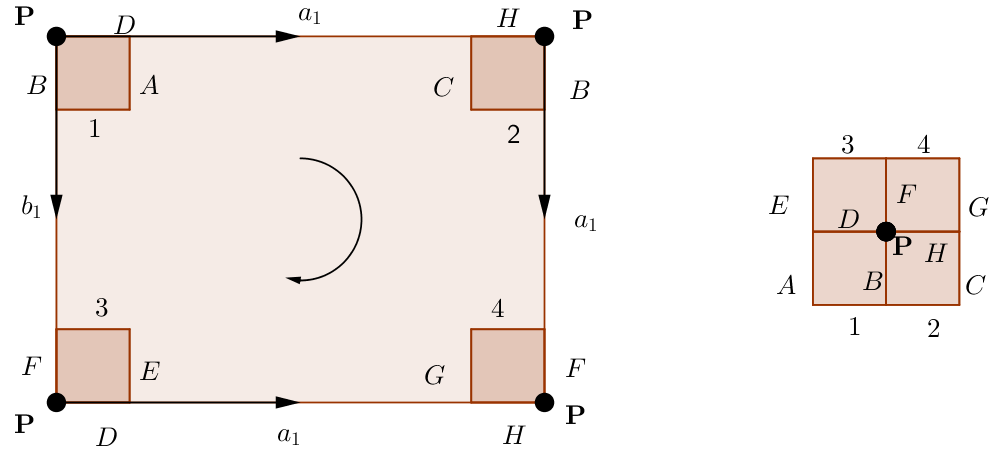
\includegraphics[scale=0.26]{entorno}
\end{figure}
%\begin{center}
%\definecolor{zzttqq}{rgb}{0.6,0.2,.}
%\definecolor{q}{rgb}{0.8,0.2,.}
%\begin{tikzpicture}[line cap=round,line join=round,>=triangle 45,x=1.0cm,y=1.0cm]
%\clip(-2.3066666666666653,-0.5) rectangle (8.872,2.5);
%\draw (0.,0.)-- (0.,2.);
%\draw (0.,2.)-- (3.,2.);
%\draw (3.,2.)-- (3.,0.);
%\draw (3.,0.)-- (0.,0.);
%\fill[fill=zzttqq,fill opacity=0.09](0.,0.)-- (0.,2.)-- (3.,2.)--(3.,0.)--cycle;
%\fill[fill=q,fill opacity=0.09](0.,2.)-- (0.,1.6133333333333342)-- (0.3866666666666657,1.6133333333333342)-- (0.3866666666666658,2.)--cycle;
%\fill[fill=q,fill opacity=0.09](3.,2.)-- (2.6,2.)--(2.6,1.6)--(3.,1.6)--cycle;
%\fill[fill=q,fill opacity=0.09](0.,0.)-- (0.41333333333333355,0.)--(0.41333333333333355,0.41333333333333344)-- (0.,0.41333333333333355)--cycle;
%\fill[fill=q,fill opacity=0.09](2.64,0.)-- (3.,0.)--(3.,0.36)-- (2.64,0.36)--cycle;
%\fill[fill=q,fill opacity=0.09](3.986666666666667,0.52)-- (5.,0.52)-- (5.,1.5333333333333328)--(3.986666666666667,1.5333333333333328)--cycle;
%\draw [color=zzttqq] (0.,2.)-- (0.,1.6133333333333342);
%\draw [color=zzttqq] (0.,1.6133333333333342)-- (0.3866666666666657,1.6133333333333342);
%\draw [color=zzttqq] (0.3866666666666657,1.6133333333333342)-- (0.3866666666666658,2.);
%\draw [color=zzttqq] (0.3866666666666658,2.)-- (0.,2.);
%\draw [color=zzttqq] (3.,2.)-- (2.6,2.);
%\draw [color=zzttqq] (2.6,2.)-- (2.6,1.6);
%\draw [color=zzttqq] (2.6,1.6)-- (3.,1.6);
%\draw [color=zzttqq] (3.,1.6)-- (3.,2.);
%\draw [color=zzttqq] (0.,0.)-- (0.41333333333333355,0.);
%\draw [color=zzttqq] (0.41333333333333355,0.)-- (0.41333333333333355,0.41333333333333344);
%\draw [color=zzttqq] (0.41333333333333355,0.41333333333333344)-- (0.,0.41333333333333355);
%\draw [color=zzttqq] (0.,0.41333333333333355)-- (0.,0.);
%\draw [color=zzttqq] (2.64,0.)-- (3.,0.);
%\draw [color=zzttqq] (3.,0.)-- (3.,0.36);
%\draw [color=zzttqq] (3.,0.36)-- (2.64,0.36);
%\draw [color=zzttqq] (2.64,0.36)-- (2.64,0.);
%\draw [->] (0.,2.) -- (1.6133333333333333,2.);
%\draw [->] (0.,0.) -- (1.68,0.);
%\draw [->] (3.,2.) -- (3.,0.8133333333333339);
%\draw [->] (0.,2.) -- (0.,0.8533333333333339);
%\draw [shift={(1.4266666666666667,1.0533333333333335)}] plot[domain=-1.5707963267948966:1.6041173226731442,variable=\t]({1.*0.48*cos(\t r)+0.*0.48*sin(\t r)},{0.*0.48*cos(\t r)+1.*0.48*sin(\t r)});
%\draw [->] (1.4266666666666667,0.5733333333333335) -- (1.04,0.626666666666667);
%\draw (3.986666666666667,0.52)-- (5.,0.52);
%\draw (5.,0.52)-- (5.,1.5333333333333328);
%\draw (5.,1.5333333333333328)-- (3.986666666666667,1.5333333333333328);
%\draw (3.986666666666667,1.5333333333333328)-- (3.986666666666667,0.52);
%\draw (4.493333333333332,1.5333333333333332)-- (4.493333333333332,0.52);
%\draw (3.986666666666667,1.0266666666666664)-- (5.,1.0266666666666664);
%\draw (-0.4,2.381333333333332) node[anchor=north west] {$\textbf{P}$};
%\draw (3.0586666666666646,2.2853333333333326) node[anchor=north west] {$\textbf{P}$};
%\draw (-0.4,-0.008) node[anchor=north west] {$\textbf{P}$};
%\draw (3.133333333333331,0.056) node[anchor=north west] {$\textbf{P}$};
%\draw (4.4,1.1546666666666665) node[anchor=north west] {$\textbf{P}$};
%\draw (1.4586666666666657,2.349333333333332) node[anchor=north west] {$a_1$};
%\draw (1.4053333333333324,0.002666666666667271) node[anchor=north west] {$a_1$};
%\draw (-0.5,1.208) node[anchor=north west] {$b_1$};
%\draw (3.112,1.1546666666666665) node[anchor=north west] {$b_1$};
%\draw (0.,1.688) node[anchor=north west] {$1$};
%\draw (2.6,1.698666666666666) node[anchor=north west] {$2$};
%\draw (0.,0.728) node[anchor=north west] {$3$};
%\draw (2.6,0.728) node[anchor=north west] {$4$};
%\draw (0.41333333333333305,1.9973333333333325) node[anchor=north west] {$A$};
%\draw (-0.5,1.976) node[anchor=north west] {$B$};
%\draw (0.,2.4) node[anchor=north west] {$D$};
%\draw (2.1,1.9546666666666659) node[anchor=north west] {$C$};
%\draw (3.0373333333333314,1.976) node[anchor=north west] {$B$};
%\draw (2.5,2.4) node[anchor=north west] {$H$};
%\draw (0.4,0.354666666666667) node[anchor=north west] {$E$};
%\draw (0.,0.07733333333333389) node[anchor=north west] {$D$};
%\draw (-0.5,0.408) node[anchor=north west] {$F$};
%\draw (2.2,0.376) node[anchor=north west] {$G$};
%\draw (3.048,0.408) node[anchor=north west] {$F$};
%\draw (2.6,0.056) node[anchor=north west] {$H$};
%\draw (4.,0.6106666666666668) node[anchor=north west] {$1$};
%\draw (4.6,0.6213333333333335) node[anchor=north west] {$2$};
%\draw (4.,1.890666666666666) node[anchor=north west] {$3$};
%\draw (4.55,1.8693333333333326) node[anchor=north west] {$4$};
%\draw (3.5,0.9306666666666666) node[anchor=north west] {$A$};
%\draw (4.2,0.9306666666666666) node[anchor=north west] {$B$};
%\draw (5.05333333333333,0.9733333333333333) node[anchor=north west] {\small{$C$}};
%\draw (3.5,1.4746666666666663) node[anchor=north west] {\small{$E$}};
%\draw (3.9,1.2293333333333332) node[anchor=north west] {\small{$D$}};
%\draw (4.2,1.485333333333333) node[anchor=north west] {\small{$F$}};
%\draw (4.712,1.24) node[anchor=north west] {\small{$H$}};
%\draw (5.064,1.4426666666666663) node[anchor=north west] {\small{$G$}};
%\begin{scriptsize}
%\draw [fill=black] (0.,0.) circle (1.5pt);
%\draw [fill=black] (0.,2.) circle (1.5pt);
%\draw [fill=black] (3.,2.) circle (1.5pt);
%\draw [fill=black] (3.,0.) circle (1.5pt);
%\draw [fill=black] (4.493333333333331,1.0266666666666666) circle (1.5pt);
%\end{scriptsize}
%\end{tikzpicture}
%\end{center}
\end{observacion}

Para que el teorema tenga sentido es necesario que todas las superficies compactas sin borde puedan ser expresadas tal como hemos definido los dos tipos. Esto es cierto también para las compactas sin borde. Por ello, tenemos el siguiente teorema.

\begin{teorema} Toda superficie compacta puede obtenerse  como un espacio cociente de un polígono fundamental.
\end{teorema}

\newpage

\begin{ej}[Botella de Klein]\label{klein}\

\definecolor{zzttqq}{rgb}{0.,0.6,0.3}
\begin{tikzpicture}[line cap=round,line join=round,>=triangle 45,x=1.0cm,y=1.0cm]
\clip(-0.5,-0.5) rectangle (13,2.5);
\fill[fill=zzttqq,fill opacity=0.1](0.,0.)-- (0.,2.)-- (3.,2.)-- (3.,0.)--cycle;
\draw (0.,0.)-- (0.,2.);
\draw (0.,2.)-- (3.,2.);
\draw (3.,2.)-- (3.,0.);
\draw (3.,0.)-- (0.,0.);
\draw [->] (3.,0.) -- (1.4733333333333327,0.);
\draw [->] (0.,0.) -- (0.,1.);
\draw [->] (0.,2.) -- (1.5133333333333332,2.);
\draw [->] (3.,0.) -- (3.,1.);
\draw [color=zzttqq] (0.332,2.)-- (0.,2.);
\draw [color=zzttqq] (0.,2.)-- (0.,1.668);
\draw [color=zzttqq] (0.,1.668)-- (0.332,1.668);
\draw [color=zzttqq] (0.332,1.668)-- (0.332,2.);
\draw [color=zzttqq] (3.,2.)-- (2.6466666666666656,2.);
\draw [color=zzttqq] (2.6466666666666656,2.)-- (2.6466666666666656,1.6466666666666656);
\draw [color=zzttqq] (2.6466666666666656,1.6466666666666656)-- (3.,1.6466666666666656);
\draw [color=zzttqq] (3.,1.6466666666666656)-- (3.,2.);
\draw [color=zzttqq] (0.,0.)-- (0.332,0.);
\draw [color=zzttqq] (0.332,0.)-- (0.332,0.332);
\draw [color=zzttqq] (0.332,0.332)-- (0.,0.332);
\draw [color=zzttqq] (0.,0.332)-- (0.,0.);
\draw [color=zzttqq] (2.6466666666666656,0.)-- (3.,0.);
\draw [color=zzttqq] (3.,0.)-- (3.,0.3533333333333342);
\draw [color=zzttqq] (3.,0.3533333333333342)-- (2.646666666666666,0.35333333333333455);
\draw [color=zzttqq] (2.646666666666666,0.35333333333333455)-- (2.6466666666666656,0.);
\draw [shift={(1.,0.)},color=zzttqq]  (0,0) --  plot[domain=0.:3.141592653589793,variable=\t]({1.*0.23866666666666592*cos(\t r)+0.*0.23866666666666592*sin(\t r)},{0.*0.23866666666666592*cos(\t r)+1.*0.23866666666666592*sin(\t r)}) -- cycle ;
\draw [shift={(2.,2.)},color=zzttqq]  (0,0) --  plot[domain=-3.141592653589793:0.,variable=\t]({1.*0.2493333333333343*cos(\t r)+0.*0.2493333333333343*sin(\t r)},{0.*0.2493333333333343*cos(\t r)+1.*0.2493333333333343*sin(\t r)}) -- cycle ; %,fill=zzttqq,fill opacity=0.0.5
\draw (-0.4,1.1426666666666665) node[anchor=north west] {$a$};
\draw (3.1,1.1426666666666665) node[anchor=north west] {$a$};
\draw (1.484,2.412) node[anchor=north west] {$b$};
\draw (1.5053333333333325,-0.0413333333333327) node[anchor=north west] {$b$};
\draw (4.342666666666665,1.2386666666666664) node[anchor=north west] {$\textit{¿Cómo aparece en el teorema de clasificación?}$};
\end{tikzpicture}

\definecolor{zzttqq}{rgb}{0.,0.6,0.3}
\begin{tikzpicture}[line cap=round,line join=round,>=triangle 45,x=1.0cm,y=1.0cm]
\clip(-0.48266666666666597,-0.5) rectangle (11.784,2.5);
\fill[fill=zzttqq,fill opacity=0.09](0.,0.)-- (0.,2.)--(3,2)--(3,0)--cycle;
\fill[fill=zzttqq,fill opacity=0.09](5.,0.)-- (5.,2.)--(6,2)--(6,0)--cycle;
\fill[fill=zzttqq,fill opacity=0.09](7.,0.)-- (7.,2.)--(8,2)--(8,0)--cycle;
\fill[fill=zzttqq,fill opacity=0.09](9.,0.)-- (9.,2.)--(10,2)--(10,0)--cycle;
\draw [color=zzttqq] (0.,0.)-- (0.,2.);
\draw [color=zzttqq] (0.,2.)-- (3.,2.);
\draw [color=zzttqq] (3.,2.)-- (3.,0.);
\draw [color=zzttqq] (3.,0.)-- (0.,0.);
\draw [->] (3.,0.) -- (1.544,0.);
\draw [->] (0.,0.) -- (0.,1.);
\draw [->] (0.,2.) -- (1.5226666666666668,2.);
\draw [->,dash pattern=on 3pt off 3pt] (3.,0.) -- (3.,1.);
\draw [dash pattern=on 3pt off 3pt] (1.,0.) -- (1.,2.);
\draw [dash pattern=on 3pt off 3pt] (2.,0.) -- (2.,2.);
\draw [->] (3.6773333333333325,0.9973333333333333) -- (4.434666666666666,0.9973333333333333);
\draw (5.,0.)-- (5.,2.);
\draw (5.,0.)-- (6.,0.);
\draw (6.,0.)-- (6.,2.);
\draw (5.,2.)-- (6.,2.);
\draw (7.,0.)-- (7.,2.);
\draw (7.,0.)-- (8.,0.);
\draw (8.,0.)-- (8.,2.);
\draw (7.,2.)-- (8.,2.);
\draw (9.,0.)-- (10.,0.);
\draw (9.,0.)-- (9.,2.);
\draw (10.,0.)-- (10.,2.);
\draw (9.,2.)-- (10.,2.);
\draw [->] (10.589333333333329,1.050666666666667) -- (11.42133333333333,1.050666666666667);
\draw [->] (5.,0.) -- (5.,1.);
\draw [->] (5.,2.) -- (5.544,2.);
\draw [->] (6.,0.) -- (6.,1.);
\draw [->] (6.,0.) -- (5.469333333333331,0.);
\draw [->] (7.,0.) -- (7.,1.);
\draw [->] (7.,2.) -- (7.506666666666664,2.);
\draw [->] (8.,0.) -- (8.,1.);
\draw [->] (8.,0.) -- (7.4533333333333305,0.);
\draw [->] (9.,0.) -- (9.,1.);
\draw [->] (9.,2.) -- (9.56533333333333,2.);
\draw [->] (10.,0.) -- (9.512,0.);
\draw [->] (10.,0.) -- (10.,1.);
\draw (-0.06666666666666611,2.352) node[anchor=north west] {$v$};
\draw (3.144,2.256) node[anchor=north west] {$v$};
\draw (-0.024,-0.016) node[anchor=north west] {$v$};
\draw (3.0053333333333327,-0.016) node[anchor=north west] {$v$};
\draw (4.6,2.224) node[anchor=north west] {$v$};
\draw (4.6,0.05866666666666784) node[anchor=north west] {$v$};
\draw (10.14133333333333,2.245333333333333) node[anchor=north west] {$v$};
\draw (10.130666666666663,0.03733333333333452) node[anchor=north west] {$v$};
\draw (-0.4,1.1893333333333338) node[anchor=north west] {$a$};
\draw (3.112,1.082666666666667) node[anchor=north west] {$a$};
\draw (1.4586666666666668,2.373333333333333) node[anchor=north west] {$b$};
\draw (1.5013333333333334,-0.005333333333332117) node[anchor=north west] {$b$};
\draw (4.5,1.1146666666666671) node[anchor=north west] {$a$};
\draw (10.194666666666663,1.210666666666667) node[anchor=north west] {$a$};
\draw (0.3,1.9893333333333332) node[anchor=north west] {$\alpha_1$};
\draw (1.3,1.9253333333333331) node[anchor=north west] {$\alpha_2$};
\draw (2.3,1.9466666666666665) node[anchor=north west] {$\alpha_3$};
\draw (0.3,0.3786666666666676) node[anchor=north west] {$\alpha_3$};
\draw (1.3,0.5) node[anchor=north west] {$\alpha_2$};
\draw (2.3,0.3573333333333343) node[anchor=north west] {$\alpha_1$};
\draw (5.3,2.32) node[anchor=north west] {$\alpha_1$};
\draw (7.3,2.309333333333333) node[anchor=north west] {$\alpha_2$};
\draw (9.3,2.3946666666666663) node[anchor=north west] {$\alpha_3$};
\draw (5.3,-0.016) node[anchor=north west] {$\alpha_3$};
\draw (7.3,-0.06933333333333207) node[anchor=north west] {$\alpha_2$};
\draw (9.3,-0.048) node[anchor=north west] {$\alpha_1$};
\draw (0.936,2.373333333333333) node[anchor=north west] {$q$};
\draw (2.013333333333333,2.341333333333333) node[anchor=north west] {$p$};
\draw (0.9893333333333336,-0.016) node[anchor=north west] {$p$};
\draw (2.088,0.026666666666667862) node[anchor=north west] {$q$};
\draw (6.034666666666665,2.341333333333333) node[anchor=north west] {$q$};
\draw (6.6,2.234666666666666) node[anchor=north west] {$q$};
\draw (8,2.266666666666666) node[anchor=north west] {$p$};
\draw (8.5,2.256) node[anchor=north west] {$p$};
\draw (6.066666666666665,0.005333333333334542) node[anchor=north west] {$p$};
\draw (6.909333333333331,0.005333333333334542) node[anchor=north west] {$p$};
\draw (8.050666666666665,0.005333333333334542) node[anchor=north west] {$q$};
\draw (8.936,-0.005333333333332117) node[anchor=north west] {$q$};
\draw [->,dash pattern=on 3pt off 3pt] (1.,0.) -- (1.,1.0186666666666673);
\draw [->,dash pattern=on 3pt off 3pt] (2.,0.) -- (2.,0.9973333333333338);
\draw (0.6,1.2) node[anchor=north west] {$d$};
\draw (1.6,1.1) node[anchor=north west] {$c$};
\draw (6.109333333333331,1.1466666666666672) node[anchor=north west] {$d$};
\draw (6.5,1.136) node[anchor=north west] {$d$};
\draw (8.12533333333333,1.0293333333333339) node[anchor=north west] {$c$};
\draw (8.6,1.061333333333334) node[anchor=north west] {$c$};
\begin{scriptsize}
\draw [fill=black] (0.,0.) circle (2.5pt);
\draw [fill=black] (0.,2.) circle (2.5pt);
\draw [fill=black] (3.,2.) circle (2.5pt);
\draw [fill=black] (3.,0.) circle (2.5pt);
\draw [fill=black] (1.,0.) circle (2.5pt);
\draw [fill=black] (1.,2.) circle (2.5pt);
\draw [fill=black] (2.,0.) circle (2.5pt);
\draw [fill=black] (2.,2.) circle (2.5pt);
\draw [fill=black] (5.,0.) circle (2.5pt);
\draw [fill=black] (5.,2.) circle (2.5pt);
\draw [fill=black] (6.,0.) circle (2.5pt);
\draw [fill=black] (6.,2.) circle (2.5pt);
\draw [fill=black] (7.,0.) circle (2.5pt);
\draw [fill=black] (7.,2.) circle (2.5pt);
\draw [fill=black] (8.,0.) circle (2.5pt);
\draw [fill=black] (8.,2.) circle (2.5pt);
\draw [fill=black] (9.,0.) circle (2.5pt);
\draw [fill=black] (10.,0.) circle (2.5pt);
\draw [fill=black] (9.,2.) circle (2.5pt);
\draw [fill=black] (10.,2.) circle (2.5pt);
\end{scriptsize}
\end{tikzpicture}

\begin{tikzpicture}[line cap=round,line join=round,>=triangle 45,x=1.0cm,y=1.0cm]
\clip(-3.252,-1) rectangle (9.014666666666665,2.5);
\fill[fill=zzttqq,fill opacity=0.09](1.,0.)-- (0.,0.)--(0,2)--(1,2)--cycle;
\fill[fill=zzttqq,fill opacity=0.09](2.,0.)-- (4.,0.)--(4,2)--(2,2)--cycle;
\draw (1.,0.)-- (0.,0.);
\draw (0.,0.)-- (0.,2.);
\draw (0.,2.)-- (1.,2.);
\draw (1.,2.)-- (1.,0.);
\draw (2.,0.)-- (4.,0.);
\draw (4.,0.)-- (4.,2.);
\draw (4.,2.)-- (2.,2.);
\draw (2.,2.)-- (2.,0.);
\draw [->] (1.,0.) -- (0.48133333333333317,0.);
\draw [->] (0.,0.) -- (0.,1.);
\draw [->] (0.,2.) -- (0.5346666666666665,2.);
\draw [->] (1.,0.) -- (1.,1.);
\draw [->] (3.,0.) -- (2.476,0.);
\draw [->] (2.,0.) -- (2.,1.);
\draw [->] (2.,2.) -- (2.550666666666666,2.);
\draw [->] (3.0093333333333327,2.) -- (3.532,2.);
\draw [->] (4.,0.) -- (3.5,0.);
\draw [->] (4.,0.) -- (4.,1.);
\draw [dash pattern=on 3pt off 3pt] (3.,0.)-- (3.0093333333333327,2.);
\draw [->,dash pattern=on 3pt off 3pt] (3.,0.) -- (3.00466656503925,0.9999782226964835);
\draw [->] (-1.332,1.2226666666666681) -- (-0.6813333333333332,1.212);
\draw (-0.4,1.158666666666668) node[anchor=north west] {$d$};
\draw (1.1,1.1) node[anchor=north west] {$c$};
\draw (1.5,1.1) node[anchor=north west] {$c$};
\draw (2.5,1.1) node[anchor=north west] {$a$};
\draw (4.193333333333333,1.148) node[anchor=north west] {$d$};
\draw (0.40666666666666773,2.364) node[anchor=north west] {$\alpha_2$};
\draw (2.4,2.310666666666669) node[anchor=north west] {$\alpha_3$};
\draw (3.4,2.3213333333333357) node[anchor=north west] {$\alpha_1$};
\draw (0.4386666666666677,0.0386666666666673) node[anchor=north west] {$\alpha_2$};
\draw (2.358666666666667,0.017333333333333954) node[anchor=north west] {$\alpha_1$};
\draw (3.35,0.006666666666667279) node[anchor=north west] {$\alpha_3$};
\draw (-0.4,2.2253333333333356) node[anchor=north west] {$q$};
\draw (1.1,2.1933333333333356) node[anchor=north west] {$p$};
\draw (-0.1586666666666654,0.006666666666667279) node[anchor=north west] {$p$};
\draw (1.1,0.006666666666667279) node[anchor=north west] {$q$};
\draw (1.6,2.204) node[anchor=north west] {$p$};
\draw (4.182666666666666,2.204) node[anchor=north west] {$q$};
\draw (1.793333333333334,0.017333333333333954) node[anchor=north west] {$q$};
\draw (4.076,0.017333333333333954) node[anchor=north west] {$p$};
\draw (2.9773333333333336,2.364) node[anchor=north west] {$v$};
\draw (2.9773333333333336,0.006666666666667279) node[anchor=north west] {$v$};
\draw (-0.5,-0.356) node[anchor=north west] {$\textit{B. Möbius}$};
\draw (2,-0.388) node[anchor=north west] {$\textit{B. Möbius}$};
\begin{scriptsize}
\draw [fill=black] (1.,0.) circle (2.5pt);
\draw [fill=black] (0.,0.) circle (2.5pt);
\draw [fill=black] (0.,2.) circle (2.5pt);
\draw [fill=black] (1.,2.) circle (2.5pt);
\draw [fill=black] (2.,0.) circle (2.5pt);
\draw [fill=black] (4.,0.) circle (2.5pt);
\draw [fill=black] (4.,2.) circle (2.5pt);
\draw [fill=black] (2.,2.) circle (2.5pt);
\draw [fill=black] (3.,0.) circle (2.5pt);
\draw [fill=black] (3.0093333333333327,2.) circle (2.5pt);
\end{scriptsize}

\end{tikzpicture}
\begin{figure}[h!]
	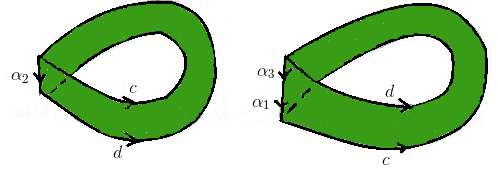
\includegraphics[scale=0.6]{m}
\end{figure}

Una botella de Klein aparece al unir dos bandas de Möbius por el borde. Ahora veremos que esto mismo le ocurre a la superficie $N_2$.



\begin{tikzpicture}[line cap=round,line join=round,>=triangle 45,x=1.0cm,y=1.0cm]
\clip(1.12,4) rectangle (16.453333333333337,6.7);
\fill[fill=zzttqq,fill opacity=0.09](2.2,6.2733333333333325)-- (2.186666666666667,4.713333333333332)--(4.773333333333334,4.7)-- (4.76,6.26)--cycle;
\fill[fill=zzttqq,fill opacity=0.09](7.64,6.1933333333333325)-- (7.653333333333335,4.7)-- (9.84,4.673333333333332)-- (7.64,6.1933333333333325)--cycle;
\draw [fill=zzttqq,fill opacity=0.09] (13.66666666666667,5.366666666666665) circle (1.1361533542812094cm);
\draw [rotate around={49.53777250790664:(13.993333333333329,5.913333333333326)},color=white,fill=white,fill opacity=1.0] (13.993333333333329,5.913333333333326) ellipse (0.49891094496497096cm and 0.4001956714537416cm);
\draw (2.2,6.2733333333333325)-- (2.186666666666667,4.713333333333332);
\draw (2.186666666666667,4.713333333333332)-- (4.773333333333334,4.7);
\draw (4.773333333333334,4.7)-- (4.76,6.26);
\draw (4.76,6.26)-- (2.2,6.2733333333333325);
\draw [->] (2.2,6.2733333333333325) -- (3.5065617794656183,6.266528324065283);
\draw [->] (4.773333333333334,4.7) -- (3.4666326575798645,4.706735570493574);
\draw [->] (2.186666666666667,4.713333333333332) -- (2.1936177258339424,5.526607255904552);
\draw [->,dash pattern=on 3pt off 3pt] (4.76,6.26) -- (4.7678616995373755,5.3401811541271);
\draw [dash pattern=on 3pt off 3pt] (2.2,6.2733333333333325)-- (4.773333333333334,4.7);
\draw [->,dash pattern=on 3pt off 3pt] (2.2,6.2733333333333325) -- (3.661388622906612,5.379841843680586);
\draw [->] (5.733333333333334,5.34) -- (6.906666666666668,5.326666666666665);
\draw (7.64,6.1933333333333325)-- (7.653333333333335,4.7);
\draw (7.653333333333335,4.7)-- (9.84,4.673333333333332);
\draw (9.84,4.673333333333332)-- (7.64,6.1933333333333325);
\draw [->] (7.64,6.1933333333333325) -- (8.793084209741181,5.396656970239425);
\draw [->] (9.84,4.673333333333332) -- (8.640015861214374,4.687967286245352);
\draw [->] (7.653333333333335,4.7) -- (7.646785173375847,5.433393915238474);
\draw [->] (10.2,5.54) -- (11.573333333333336,5.5266666666666655);
\draw(13.66666666666667,5.366666666666665) circle (1.1361533542812094cm);
\draw [rotate around={49.53777250790664:(13.993333333333329,5.913333333333326)}] (13.993333333333329,5.913333333333326) ellipse (0.49891094496497096cm and 0.4001956714537416cm);
\draw [->] (13.598650992822087,5.619220376162084) -- (13.777410756858053,5.472773823874067);
\draw [->] (12.558507606500173,5.617321692180517) -- (12.671690150363672,5.915179361551654);
\draw [->] (14.774825726833168,5.116011641152815) -- (14.706006932353207,4.907737198701182);
\draw (1.8,6.686666666666666) node[anchor=north west] {$P$};
\draw (4.9733333333333345,6.553333333333332) node[anchor=north west] {$P$};

\draw (2.04,4.686666666666666) node[anchor=north west] {$P$};
\draw (4.906666666666668,4.74) node[anchor=north west] {$P$};
\draw (7.,6.433333333333332) node[anchor=north west] {$P$};
\draw (7.3,4.633333333333333) node[anchor=north west] {$P$};
\draw (9.8,4.66) node[anchor=north west] {$P$};
\draw (12.693333333333335,4.446666666666665) node[anchor=north west] {$P$};
\draw (14.58666666666667,6.713333333333332) node[anchor=north west] {$P$};
\draw (3.426666666666667,6.713333333333332) node[anchor=north west] {$a_1$};
\draw (5.,5.5666666666666655) node[anchor=north west] {$a_1$};
\draw (3.386666666666667,4.62) node[anchor=north west] {$a_2$};
\draw (1.6,5.633333333333332) node[anchor=north west] {$a_2$};
\draw (3.52,5.913333333333332) node[anchor=north west] {$\alpha$};
\draw (8.72,5.833333333333332) node[anchor=north west] {$\alpha$};
\draw (8.4,4.5266666666666655) node[anchor=north west] {$a_2$};
\draw (7,5.54) node[anchor=north west] {$a_2$};
\draw (14.6,4.66) node[anchor=north west] {$a_2$};
\draw (12,6.06) node[anchor=north west] {$a_2$};
\draw (13.56,5.5) node[anchor=north west] {$\alpha$};
\begin{scriptsize}
\draw [fill=black] (2.2,6.2733333333333325) circle (2.5pt);
\draw [fill=black] (2.186666666666667,4.713333333333332) circle (2.5pt);
\draw [fill=black] (4.773333333333334,4.7) circle (2.5pt);
\draw [fill=black] (4.76,6.26) circle (2.5pt);
\draw [fill=black] (7.64,6.1933333333333325) circle (2.5pt);
\draw [fill=black] (7.653333333333335,4.7) circle (2.5pt);
\draw [fill=black] (9.84,4.673333333333332) circle (2.5pt);
\draw [fill=black] (14.333333333333336,6.286666666666665) circle (2.5pt);
\draw [fill=black] (13.,4.446666666666667) circle (2.5pt);
\end{scriptsize}
\end{tikzpicture}
Nos hemos fijado solo en una mitad, la otra daría el mismo resultado. Esto es, $N_2$ es la unión por el borde de dos planos proyectivos con un agujero. Ahora bien, 
\end{ej}
\begin{observacion}[Importante] El plano proyectivo con un agujero es una banda de Möbius cuyo borde 
es el borde del agujero.

\definecolor{zzttqq}{rgb}{0.,0.6,0.3}
\begin{tikzpicture}[line cap=round,line join=round,>=triangle 45,x=1.0cm,y=1.0cm]
\clip(0.2866666666666677,1) rectangle (14.226060606060612,7);
\fill[fill=zzttqq,fill opacity=0.09](1.18,6.553333333333332)-- (1.1666666666666665,5.14)-- (2.94,5.126666666666666)--cycle;
\fill[fill=zzttqq,fill opacity=0.09](4.5,5.58)-- (5.153333333333334,6.433333333333332)-- (5.713333333333335,5.54)--cycle;
\fill[fill=zzttqq,fill opacity=0.09](6.02,4.82)-- (6.726666666666668,5.673333333333332)-- (7.286666666666668,4.766666666666666)--cycle;
\fill[fill=zzttqq,fill opacity=0.09](9.793333333333335,5.5266666666666655)-- (10.713333333333335,6.34)--(11.713333333333336,5.353333333333333)--(10.7,4.406666666666665)--cycle;
\fill[fill=zzttqq,fill opacity=0.09](1.5533333333333332,2.9933333333333327)-- (3.6466666666666674,2.9933333333333327)--(3.6466666666666674,1.7)--(1.54,1.7)--cycle;
\draw (1.18,6.553333333333332)-- (1.1666666666666665,5.14);
\draw (1.18,6.553333333333332)-- (2.94,5.126666666666666);
\draw (1.1666666666666665,5.14)-- (2.94,5.126666666666666);
\draw [->] (2.94,5.126666666666666) -- (1.9189467240554758,5.134343758967001);
\draw [->] (1.1666666666666665,5.14) -- (1.1733333333333333,5.846666666666666);
\draw [->] (1.18,6.553333333333332) -- (1.7316572576455505,6.10615661690853);
\draw [->] (1.7316572576455505,6.10615661690853) -- (2.1909043050600907,5.733888176958865);
\draw [->] (2.1909043050600907,5.733888176958865) -- (2.664719980604718,5.349810318752235);
\draw [->] (3.,6.) -- (4.326666666666667,5.98);
\draw [dash pattern=on 3pt off 3pt] (1.1666666666666665,5.14)-- (2.1909043050600907,5.733888176958865);
\draw [->,dash pattern=on 3pt off 3pt] (1.1666666666666665,5.14) -- (1.8691025829679326,5.547296480938683);
\draw (4.5,5.58)-- (5.153333333333334,6.433333333333332);
\draw (5.153333333333334,6.433333333333332)-- (5.713333333333335,5.54);
\draw (4.5,5.58)-- (5.713333333333335,5.54);
\draw (6.02,4.82)-- (6.726666666666668,5.673333333333332);
\draw (6.726666666666668,5.673333333333332)-- (7.286666666666668,4.766666666666666);
\draw (6.02,4.82)-- (7.286666666666668,4.766666666666666);
\draw [->] (7.42,5.94) -- (8.846666666666668,5.9);
\draw (9.793333333333335,5.5266666666666655)-- (10.713333333333335,6.34);
\draw (10.713333333333335,6.34)-- (11.713333333333336,5.353333333333333);
\draw (11.713333333333336,5.353333333333333)-- (10.7,4.406666666666665);
\draw (10.7,4.406666666666665)-- (9.793333333333335,5.5266666666666655);
\draw (1.5533333333333332,2.9933333333333327)-- (3.6466666666666674,2.9933333333333327);
\draw (1.5533333333333332,2.9933333333333327)-- (1.54,1.7);
\draw (1.54,1.7)-- (3.6466666666666674,1.7);
\draw (3.6466666666666674,1.7)-- (3.6466666666666674,2.9933333333333327);
\draw [->] (4.5,5.58) -- (4.859800933764302,6.049944076753373);
\draw [->] (4.5,5.58) -- (5.113106554081223,5.5597876960193);
\draw [->] (5.153333333333334,6.433333333333332) -- (5.450573058265364,5.959165200703666);
\draw [->] (6.726666666666668,5.673333333333332) -- (7.005264036735547,5.222270924650385);
\draw [->] (7.286666666666668,4.766666666666666) -- (6.647238874755744,4.793589942115547);
\draw [->,dash pattern=on 3pt off 3pt] (6.02,4.82) -- (6.398867487328019,5.277500362056474);
\draw [dash pattern=on 3pt off 3pt] (11.713333333333336,5.353333333333333)-- (9.793333333333335,5.5266666666666655);
\draw [->,dash pattern=on 3pt off 3pt] (11.713333333333336,5.353333333333333) -- (10.686608626325443,5.4460237582715445);
\draw [->] (9.793333333333335,5.5266666666666655) -- (10.275578515644543,5.952999364072228);
\draw [->] (11.713333333333336,5.353333333333333) -- (11.168671031289131,4.844504077476247);


\draw [->] (1.54,1.7) -- (1.5478836827359674,2.4647172253888505);
\draw [->] (3.6466666666666674,2.9933333333333327) -- (3.6466666666666674,2.258787878787878);

\draw (4.4,6.5) node[anchor=north west] {$a_2$};
\draw (0.6,6.792121212121211) node[anchor=north west] {$P$};
\draw (1.0381818181818194,5.1072727272727265) node[anchor=north west] {$P$};
\draw (3.0381818181818203,5.1072727272727265) node[anchor=north west] {$P$};
\draw (0.6,5.967878787878787) node[anchor=north west] {$a_2$};
\draw (1.8,5.1072727272727265) node[anchor=north west] {$a_2$};
\draw (2.23818181818182,6.1496969696969686) node[anchor=north west] {$\alpha$};
\draw (1.66848484848485,6.598181818181817) node[anchor=north west] {$\alpha_1$};
\draw (2.601818181818184,5.786060606060605) node[anchor=north west] {$\alpha_2$};
\draw (1.5472727272727287,6) node[anchor=north west] {$\beta$};
\draw (4.286666666666669,5.5678787878787865) node[anchor=north west] {$P$};
\draw (5.08666666666667,6.913333333333332) node[anchor=north west] {$P$};
\draw (5.595757575757578,6.27090909090909) node[anchor=north west] {$\alpha_1$};
\draw (4.9,5.6) node[anchor=north west] {$\beta$};
\draw (6.,5.6) node[anchor=north west] {$\beta$};
\draw (5.838181818181821,4.852727272727272) node[anchor=north west] {$P$};
\draw (7.353333333333336,4.8163636363636355) node[anchor=north west] {$P$};
\draw (6.613939393939397,4.743636363636362) node[anchor=north west] {$a_2$};
\draw (7.135151515151518,5.519393939393939) node[anchor=north west] {$\alpha_2$};
\draw (9.8,6.4) node[anchor=north west] {$\beta$};
\draw (11.377575757575762,4.961818181818181) node[anchor=north west] {$\beta$};
\draw (11.3,6.113333333333332) node[anchor=north west] {$\alpha_2$};
\draw (9.8,4.949696969696968) node[anchor=north west] {$\alpha_1$};
\draw (10.723030303030308,5.410303030303029) node[anchor=north west] {$a_2$};
\draw (1.,2.573939393939393) node[anchor=north west] {$\beta$};
\draw (3.7,2.586060606060605) node[anchor=north west] {$\beta$};
\draw (2.3351515151515168,3.4587878787878776) node[anchor=north west] {$\alpha_1$};
\draw (2.444242424242426,1.6284848484848473) node[anchor=north west] {$\alpha_2$};
\draw (12.298787878787884,5.507272727272726) node[anchor=north west] {$\equiv$};
\draw (4.310909090909093,2.5375757575757563) node[anchor=north west] {$\equiv\textit{Banda de Möbius con borde }\alpha=\alpha_1\cup\alpha_2$};
\draw (0.6,2.5618181818181807) node[anchor=north west] {$\equiv$};
\draw [->] (10.713333333333335,6.34) -- (11.25,5.8);
\draw [->] (9.793333333333335,5.5266666666666655) -- (10.2,5.03);
\begin{scriptsize}
\draw [fill=black] (1.18,6.553333333333332) circle (2.5pt);
\draw [fill=black] (1.1666666666666665,5.14) circle (2.5pt);
\draw [fill=black] (2.94,5.126666666666666) circle (2.5pt);
\draw [fill=black] (4.5,5.58) circle (2.5pt);
\draw [fill=black] (5.153333333333334,6.433333333333332) circle (2.5pt);
\draw [color=black] (5.713333333333335,5.54) circle (2.5pt);
\draw [fill=black] (6.02,4.82) circle (2.5pt);
\draw [color=black] (6.726666666666668,5.673333333333332) circle (2.5pt);
\draw [fill=black] (7.286666666666668,4.766666666666666) circle (2.5pt);
\draw [fill=black] (9.793333333333335,5.5266666666666655) circle (2.5pt);
\draw [color=black] (10.713333333333335,6.34) circle (2.5pt);
\draw [fill=black] (11.713333333333336,5.353333333333333) circle (2.5pt);
\draw [color=black] (10.7,4.406666666666665) circle (2.5pt);
\end{scriptsize}
\end{tikzpicture}

Luego la botella de Klein resulta ser homeomorfa al modelo $N_2$.
\end{observacion}

\section{Suma Conexa}

Veamos con más detalle la operación que hemos realizado para demostrar que $N_2$ es la botella de Klein.

\begin{defi}
La \textbf{suma conexa} de dos superficies compactas sin borde $S$ y $S'$ es una nueva superficie compacta sin borde $S\# S'$ que resulta al eliminar un disco abierto en cada una de ellas y pegarlas por las circunferencias de los bordes. Más formalmente, si tenemos dos discos cerrados $D\subseteq S$ y $D'\subseteq S'$, podemos considerar un homeomorfismo $f\func{\partial D}{\partial D'}$. Entonces la suma conexa es el cociente $(S\setminus \mathring{D})\sqcup_f(S'\setminus \mathring{D'})$.
\end{defi}

\begin{nota} La suma conexa no depende de qué disco se elimine ni del tipo de homeomorfismo.
\end{nota}

\begin{propi} La suma conexa cumple las siguientes propiedades:
\begin{enumerate}
\item Es conmutativa.
\item Es asociativa.
\item $S^2$ es el elemento neutro.
\end{enumerate}
Estas propiedades dotan al conjunto de superficies compactas sin borde de estructura de monoide abeliano.
\end{propi}

\begin{ej}
La esfera $S^2$ actúa como elemento neutro de la suma conexa. Esto es, si $M$ una superficie, 
$M\# S^2$ es homeomorfa a $M$ ya que $S^2$ con un agujero es homeomorfa a un disco, como vemos en el siguiente dibujo.
\begin{figure}[h!]
	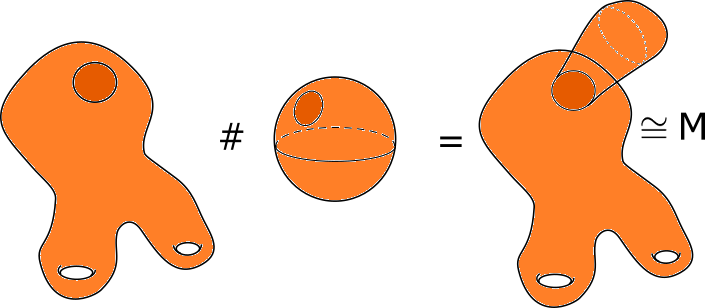
\includegraphics[scale=0.5]{text4248}
\end{figure}
\end{ej}

Veamos ahora cómo es la suma conexa de los tipos de superficies presentados.

\subsection{Tipo I}

\begin{flushleft}
$M_2=a^{}_1 b^{}_1 a^{-1}_1 b^{-1}_1 a^{}_2 b^{}_2 a^{-1}_2 b^{-1}_2$.

\definecolor{ffffff}{rgb}{0.6,0.2,0.}
\definecolor{uuuuuu}{rgb}{0.7,0.4,0.}
\begin{tikzpicture}[line cap=round,line join=round,>=triangle 45,x=1.0cm,y=1.0cm]
\clip(-1.9528215774878441,-5.848675592584895) rectangle (11.17409949375901,0.4138149713873497);
\fill[color=uuuuuu,fill=uuuuuu,fill opacity=0.1](1.,0.) -- (0.,0.) -- (-0.7071067811865475,-0.7071067811865474) -- (-0.7071067811865475,-1.7071067811865472) -- (0.,-2.414213562373095) -- (1.,-2.414213562373095) -- (1.7071067811865475,-1.7071067811865477) -- (1.7071067811865477,-0.7071067811865478) -- cycle;
\fill[color=uuuuuu,fill=uuuuuu,fill opacity=0.1] (0.,0.) -- (-0.7071067811865475,-0.7071067811865474) -- (-0.7071067811865475,-1.7071067811865472) -- (0.,-2.414213562373095) -- (1.,-2.414213562373095) -- (1.7071067811865475,-1.7071067811865477) -- (1.7071067811865477,-0.7071067811865478) -- (1.,0.) -- cycle;
\fill[color=uuuuuu,fill=uuuuuu,fill opacity=0.1] (3.766666666666668,0.) -- (2.9933333333333345,-0.7071067811865478) -- (2.9933333333333345,-1.7071067811865477) -- (3.766666666666668,-2.414213562373095) -- (4.753333333333335,-2.414213562373095) -- cycle;
\fill[color=uuuuuu,fill=uuuuuu,fill opacity=0.1] (4.,0.) -- (5.,0.) -- (5.753333333333334,-0.7071067811865478) -- (5.753333333333334,-1.7071067811865477) -- (4.986666666666666,-2.414213562373095) -- cycle;
\fill[color=uuuuuu,fill=uuuuuu,fill opacity=0.1] (5.2,-3.8) -- (3.6,-3.8) -- (3.6,-5.4) -- (5.2,-5.4) -- cycle;
\fill[color=uuuuuu,fill=uuuuuu,fill opacity=0.1] (7.6,-0.4) -- (7.6,-2.) -- (9.2,-2.) -- (9.2,-0.4) -- cycle;
\draw (1.,0.)-- (0.,0.);
\draw (0.,0.)-- (-0.7071067811865475,-0.7071067811865474);
\draw (-0.7071067811865475,-0.7071067811865474)-- (-0.7071067811865475,-1.7071067811865472);
\draw (-0.7071067811865475,-1.7071067811865472)-- (0.,-2.414213562373095);
\draw (0.,-2.414213562373095)-- (1.,-2.414213562373095);
\draw (1.,-2.414213562373095)-- (1.7071067811865475,-1.7071067811865477);
\draw (1.7071067811865475,-1.7071067811865477)-- (1.7071067811865477,-0.7071067811865478);
\draw (1.7071067811865477,-0.7071067811865478)-- (1.,0.);
\draw [dash pattern=on 3pt off 3pt] (0.,0.)-- (1.,-2.414213562373095);
\draw [->,dash pattern=on 3pt off 3pt] (0.,0.) -- (0.5449628423723549,-1.3156566850447307);
\draw [->] (1.8866666666666674,-1.1333333333333306) -- (2.62,-1.1333333333333306);
\draw (2.9933333333333345,-0.7071067811865478)-- (2.9933333333333345,-1.7071067811865477);
\draw (2.9933333333333345,-0.7071067811865478)-- (3.766666666666668,0.);
\draw (2.9933333333333345,-1.7071067811865477)-- (3.766666666666668,-2.414213562373095);
\draw (3.766666666666668,-2.414213562373095)-- (4.753333333333335,-2.414213562373095);
\draw [dash pattern=on 3pt off 3pt] (3.766666666666668,0.)-- (4.753333333333335,-2.414213562373095);
\draw [dash pattern=on 3pt off 3pt] (4.,0.)-- (4.986666666666666,-2.414213562373095);
\draw (4.,0.)-- (5.,0.);
\draw (5.,0.)-- (5.753333333333334,-0.7071067811865478);
\draw (5.753333333333334,-0.7071067811865478)-- (5.753333333333334,-1.7071067811865477);
\draw (5.753333333333334,-1.7071067811865477)-- (4.986666666666666,-2.414213562373095);
\draw [->] (6.246666666666669,-1.08) -- (7.193333333333336,-1.0933333333333306);
\draw [->] (4.273333333333334,-2.693333333333329) -- (4.273333333333334,-3.453333333333328);
\draw (0.5938474134066074,-0.8710952922003012) node[anchor=north west] {$\alpha$};
\draw (3.858214029007677,-1.0794591187280285) node[anchor=north west] {$\alpha$};
\draw (4.645366262556871,-0.9289741329024477) node[anchor=north west] {$\alpha$};
\draw [->] (0.,0.) -- (-0.43,-0.43);
\draw [->] (0.,0.) -- (0.6066666666666671,0.);
\draw [->] (-0.7071067811865475,-0.7071067811865474) -- (-0.7071067811865475,-1.2666666666666637);
\draw [->] (1.,0.) -- (1.4033333333333335,-0.4033333333333336);
\draw [->] (1.,-2.414213562373095) -- (0.42,-2.414213562373095);
\draw [->] (1.7071067811865475,-1.7071067811865477) -- (1.7071067811865477,-1.1333333333333306);
\draw [->] (1.,-2.414213562373095) -- (1.4104401145198828,-2.003773447853212);
\draw [->] (0.,-2.414213562373095) -- (-0.37044011451988273,-2.043773447853212);
\draw [->] (3.766666666666668,0.) -- (3.333839864111777,-0.39576047478343235);
\draw [->] (2.9933333333333345,-0.7071067811865478) -- (2.9933333333333345,-1.3733333333333304);
\draw [->] (3.766666666666668,-2.414213562373095) -- (3.3273833656823384,-2.0125495093713313);
\draw [->] (4.753333333333335,-2.414213562373095) -- (4.18,-2.414213562373095);
\draw [->] (4.986666666666666,-2.414213562373095) -- (5.388388668513538,-2.043700060210803);
\draw [->] (5.753333333333334,-1.7071067811865477) -- (5.753333333333334,-1.0003745192473548);
\draw [->] (4.,0.) -- (4.66,0.);
\draw [->] (5.,0.) -- (5.4267343208322085,-0.40054875932587214);
\draw (8.222278617949533,-1.426732162940907) node[anchor=north west] {$\alpha$};
\draw (4.112880928097122,-4.64479570598025) node[anchor=north west] {$\alpha$};
\draw (5.409366959825206,-3.846067704290628) node[anchor=north west] {$\text{Toro con un agujero}$};
\draw (7.828702501174935,-2.5264301362816894) node[anchor=north west] {$\text{Toro con un agujero}$};
\draw (0.4,0.4) node[anchor=north west] {$a_1$};
\draw (1.4,0.) node[anchor=north west] {$b_1$};
\draw (1.7,-1.1) node[anchor=north west] {$a_1$};
\draw (1.3,-1.9) node[anchor=north west] {$b_1$};
\draw (-0.8,0.1) node[anchor=north west] {$b_2$};
\draw (-1.3,-1.021580278025882) node[anchor=north west] {$a_2$};
\draw (-0.7,-1.9707932655410836) node[anchor=north west] {$b_2$};
\draw (0.4202108913001675,-2.45) node[anchor=north west] {$a_2$};
\draw (8.291733226792108,0.12442076787661749) node[anchor=north west] {$b_1$};
\draw (8.500097053319836,-2.02867210624323) node[anchor=north west] {$b_1$};
\draw (9.345128127571178,-0.9637014373237356) node[anchor=north west] {$a_1$};
\draw (7.1,-0.9058225966215891) node[anchor=north west] {$a_1$};
\draw (4.263365913922703,-3.3483096742521687) node[anchor=north west] {$b_2$};
\draw (4.4717297404504315,-5.350917562546436) node[anchor=north west] {$b_2$};
\draw (3.,-4.448007647592951) node[anchor=north west] {$a_2$};
\draw (5.2,-4.47115918387381) node[anchor=north west] {$a_2$};
\draw [color=uuuuuu] (0.,0.)-- (-0.7071067811865475,-0.7071067811865474);
\draw [color=uuuuuu] (-0.7071067811865475,-0.7071067811865474)-- (-0.7071067811865475,-1.7071067811865472);
\draw [color=uuuuuu] (-0.7071067811865475,-1.7071067811865472)-- (0.,-2.414213562373095);
\draw [color=uuuuuu] (0.,-2.414213562373095)-- (1.,-2.414213562373095);
\draw [color=uuuuuu] (1.,-2.414213562373095)-- (1.7071067811865475,-1.7071067811865477);
\draw [color=uuuuuu] (1.7071067811865475,-1.7071067811865477)-- (1.7071067811865477,-0.7071067811865478);
\draw [color=uuuuuu] (1.7071067811865477,-0.7071067811865478)-- (1.,0.);
\draw [color=uuuuuu] (1.,0.)-- (0.,0.);
\draw [color=uuuuuu] (3.766666666666668,0.)-- (2.9933333333333345,-0.7071067811865478);
\draw [color=uuuuuu] (2.9933333333333345,-0.7071067811865478)-- (2.9933333333333345,-1.7071067811865477);
\draw [color=uuuuuu] (2.9933333333333345,-1.7071067811865477)-- (3.766666666666668,-2.414213562373095);
\draw [color=uuuuuu] (3.766666666666668,-2.414213562373095)-- (4.753333333333335,-2.414213562373095);
\draw [color=uuuuuu] (4.753333333333335,-2.414213562373095)-- (3.766666666666668,0.);
\draw [color=uuuuuu] (4.,0.)-- (5.,0.);
\draw [color=uuuuuu] (5.,0.)-- (5.753333333333334,-0.7071067811865478);
\draw [color=uuuuuu] (5.753333333333334,-0.7071067811865478)-- (5.753333333333334,-1.7071067811865477);
\draw [color=uuuuuu] (5.753333333333334,-1.7071067811865477)-- (4.986666666666666,-2.414213562373095);
\draw [color=uuuuuu] (4.986666666666666,-2.414213562373095)-- (4.,0.);
\draw [color=uuuuuu] (5.2,-3.8)-- (3.6,-3.8);
\draw [color=uuuuuu] (3.6,-3.8)-- (3.6,-5.4);
\draw [color=uuuuuu] (3.6,-5.4)-- (5.2,-5.4);
\draw [color=uuuuuu] (5.2,-5.4)-- (5.2,-3.8);
\draw [color=uuuuuu] (7.6,-0.4)-- (7.6,-2.);
\draw [color=uuuuuu] (7.6,-2.)-- (9.2,-2.);
\draw [color=uuuuuu] (9.2,-2.)-- (9.2,-0.4);
\draw [color=uuuuuu] (9.2,-0.4)-- (7.6,-0.4);
\draw [->] (7.6,-1.982369033681513) -- (7.6,-1.1720652638514628);
\draw [->] (7.6,-0.4) -- (8.500097053319836,-0.39648879844270046);
\draw [->] (9.2,-2.) -- (9.2,-1.1604894957110334);
\draw [->] (7.6,-1.982369033681513) -- (8.500097053319836,-2.);
\draw [->] (3.6,-3.8) -- (4.437002436029143,-3.8);
\draw [->] (3.6,-5.3856448669677235) -- (3.6,-4.62164416969939);
\draw [->] (5.2,-5.4) -- (5.2,-4.610068401558961);
\draw [->] (3.6,-5.3856448669677235) -- (4.437002436029143,-5.4);
\draw [rotate around={-140.5619342704202:(7.8562804480481105,-1.7889933448714954)},color=white,fill=white,fill opacity=1.0] (7.8562804480481105,-1.7889933448714954) ellipse (0.3319698907258063cm and 0.07214241828133117cm);
\draw [rotate around={-140.56193427043104:(7.856280448048509,-1.7889933448711708)}] (7.856280448048509,-1.7889933448711708) ellipse (0.3319698907262402cm and 0.07214241828131902cm);
\draw [rotate around={-134.03424022452825:(3.811582829009906,-5.179998629928109)},color=white,fill=white,fill opacity=1.0] (3.811582829009906,-5.179998629928109) ellipse (0.305256410926976cm and 0.06539711032373638cm);
\draw [rotate around={-134.03424022450557:(3.811582829009364,-5.179998629928732)}] (3.811582829009364,-5.179998629928732) ellipse (0.305256410926218cm and 0.06539711032380609cm);
\begin{scriptsize}
\draw [fill=black] (1.,0.) circle (2.5pt);
\draw [fill=black] (0.,0.) circle (2.5pt);
\draw [fill=black] (-0.7071067811865475,-0.7071067811865474) circle (2.5pt);
\draw [fill=black] (-0.7071067811865475,-1.7071067811865472) circle (2.5pt);
\draw [fill=black] (0.,-2.414213562373095) circle (2.5pt);
\draw [fill=black] (1.,-2.414213562373095) circle (2.5pt);
\draw [fill=black] (1.7071067811865475,-1.7071067811865477) circle (2.5pt);
\draw [fill=black] (1.7071067811865477,-0.7071067811865478) circle (2.5pt);
\draw [fill=black] (2.9933333333333345,-0.7071067811865478) circle (2.5pt);
\draw [fill=black] (2.9933333333333345,-1.7071067811865477) circle (2.5pt);
\draw [fill=black] (3.766666666666668,0.) circle (2.5pt);
\draw [fill=black] (3.766666666666668,-2.414213562373095) circle (2.5pt);
\draw [fill=black] (4.753333333333335,-2.414213562373095) circle (2.5pt);
\draw [fill=black] (4.,0.) circle (2.5pt);
\draw [fill=black] (4.986666666666666,-2.414213562373095) circle (2.5pt);
\draw [fill=black] (5.,0.) circle (2.5pt);
\draw [fill=black] (5.753333333333334,-0.7071067811865478) circle (2.5pt);
\draw [fill=black] (5.753333333333334,-1.7071067811865477) circle (2.5pt);

\end{scriptsize}
\end{tikzpicture}
\begin{figure}[h!]
	$M_1\# M_1=M_2$
\includegraphics[scale=0.4]{m2}
\end{figure}\

$M_2\equiv$ Pegar dos toros ($M_1$) con un agujero por el borde del agujero.\\
$\ \vdots$\\
$M_n\equiv$ Pegar $M_{n-1}$ con agujero con $M_1$ con aujero por el borde del agujero. Es decir, $M_n=M_1\#\dots\# M_1$  ($n$ veces).
\end{flushleft}\definecolor{ffffff}{rgb}{1.,1.,1.}


%\newpage
\subsection{Tipo II}

Ya hemos visto en el ejemplo \ref{klein} que $N_2$ (botella de Klein) es la suma conexa de dos copias del plano proyectivo $\Pro_2\R$. Si hacemos $N_1=\Pro_2\R$ tenemos en general:

\begin{flushleft}
$N_n=N_{n-1}\#N_1=N_1\#\dots\# N_1$ ($n$ veces).

\definecolor{ffffff}{rgb}{1.,1.,1.}
\definecolor{qqffqq}{rgb}{0.,1.,0.}
\begin{tikzpicture}[line cap=round,line join=round,>=triangle 45,x=1.0cm,y=1.0cm]
\clip(-2.16,-0.5) rectangle (12.02666666666667,3.5);
\fill[color=ffffff,fill=ffffff,fill opacity=0.1] (5.626666666666666,2.98) -- (4.333333333333333,2.9666666666666655) -- (4.991547005383793,1.853273811105459) -- cycle;
\fill[color=ffffff,fill=ffffff,fill opacity=0.1] (5.626666666666666,2.98) -- (4.333333333333333,2.9666666666666655) -- (4.991547005383793,1.853273811105459) -- cycle;
\fill[color=qqffqq,fill=qqffqq,fill opacity=0.1] (0.52,2.86) -- (2.,3.) -- (3.0133333333333336,2.353333333333332) -- (2.4133333333333336,1.02) -- (1.1733333333333331,0.34) -- cycle;
\fill[color=qqffqq,fill=qqffqq,fill opacity=0.1] (4.333333333333333,2.9666666666666655) -- (5.626666666666666,2.98) -- (4.991547005383793,1.853273811105459) -- cycle;
\fill[color=qqffqq,fill=qqffqq,fill opacity=0.1] (3.9733333333333327,0.7333333333333333) -- (5.613333333333333,0.6066666666666658) -- (5.28,-0.15333333333333407) -- (4.293333333333333,-0.16666666666666669) -- cycle;
\draw [shift={(4.793333333333333,0.67)},dash pattern=on 3pt off 3pt,color=qqffqq,fill=qqffqq,fill opacity=0.10000000149011612]  plot[domain=-0.07708273987648973:3.064509913713303,variable=\t]({1.*0.822442162775664*cos(\t r)+0.*0.822442162775664*sin(\t r)},{0.*0.822442162775664*cos(\t r)+1.*0.822442162775664*sin(\t r)});
\draw [shift={(0.8466666666666666,1.6)},dash pattern=on 3pt off 3pt,color=qqffqq,fill=qqffqq,fill opacity=0.10000000149011612]  plot[domain=1.8244704229335393:4.966063076523333,variable=\t]({1.*1.3016570635582596*cos(\t r)+0.*1.3016570635582596*sin(\t r)},{0.*1.3016570635582596*cos(\t r)+1.*1.3016570635582596*sin(\t r)});
\draw (0.52,2.86)-- (2.,3.);
\draw (2.,3.)-- (3.0133333333333336,2.353333333333332);
\draw (3.0133333333333336,2.353333333333332)-- (2.4133333333333336,1.02);
\draw (2.4133333333333336,1.02)-- (1.1733333333333331,0.34);
\draw [shift={(0.8466666666666666,1.6)},dash pattern=on 3pt off 3pt]  plot[domain=1.8244704229335393:4.966063076523333,variable=\t]({1.*1.3016570635582596*cos(\t r)+0.*1.3016570635582596*sin(\t r)},{0.*1.3016570635582596*cos(\t r)+1.*1.3016570635582596*sin(\t r)});
\draw [dash pattern=on 3pt off 3pt] (0.52,2.86)-- (3.0133333333333336,2.353333333333332);
\draw [->,dash pattern=on 3pt off 3pt] (0.52,2.86) -- (1.9831463122145017,2.5626761504590845);
\draw [color=ffffff] (5.626666666666666,2.98)-- (4.333333333333333,2.9666666666666655);
\draw [color=ffffff] (4.333333333333333,2.9666666666666655)-- (4.991547005383793,1.853273811105459);
\draw [color=ffffff] (4.991547005383793,1.853273811105459)-- (5.626666666666666,2.98);
\draw (4.333333333333333,2.9666666666666655)-- (5.626666666666666,2.98);
\draw (5.626666666666666,2.98)-- (4.991547005383793,1.853273811105459);
\draw (4.991547005383793,1.853273811105459)-- (4.333333333333333,2.9666666666666655);
\draw (3.9733333333333327,0.7333333333333333)-- (4.293333333333333,-0.16666666666666669);
\draw (4.293333333333333,-0.16666666666666669)-- (5.28,-0.15333333333333407);
\draw (5.28,-0.15333333333333407)-- (5.613333333333333,0.6066666666666658);
\draw [shift={(4.793333333333333,0.67)},dash pattern=on 3pt off 3pt]  plot[domain=-0.07708273987648973:3.064509913713303,variable=\t]({1.*0.822442162775664*cos(\t r)+0.*0.822442162775664*sin(\t r)},{0.*0.822442162775664*cos(\t r)+1.*0.822442162775664*sin(\t r)});
\draw [->] (0.52,2.86) -- (1.39969592760181,2.943214479638009);
\draw [->] (2.,3.) -- (2.617636842698817,2.605850172751412);
\draw [->] (3.0133333333333336,2.353333333333332) -- (2.6455994455994456,1.5361469161469152);
\draw [->] (2.4133333333333336,1.02) -- (1.6799146666666658,0.6178026666666663);
\draw [->] (4.333333333333333,2.9666666666666655) -- (5.0002727594757355,2.9735423308537023);
\draw [->] (5.626666666666666,2.98) -- (5.281439295314369,2.367553646756639);
\draw [->] (5.28,-0.15333333333333407) -- (4.693080153368632,-0.16126468261213595);
\draw [->] (4.293333333333333,-0.16666666666666669) -- (4.112453602221248,0.3420575770860735);
\draw (4.3,2.5) node[anchor=north west] {$\alpha$};
\draw (5.4,0.3) node[anchor=north west] {$\alpha$};
\draw (1.0933333333333328,3.42) node[anchor=north west] {$a_1$};
\draw (2.6,1.8466666666666647) node[anchor=north west] {$a_2$};
\draw (2.546666666666667,3.) node[anchor=north west] {$a_1$};
\draw (1.84,0.806666666666665) node[anchor=north west] {$a_2$};
\draw (4.84,3.46) node[anchor=north west] {$a_1$};
\draw (5.453333333333334,2.5933333333333315) node[anchor=north west] {$a_1$};
\draw (4.68,-0.1) node[anchor=north west] {$a_2$};
\draw (3.6,0.5133333333333318) node[anchor=north west] {$a_2$};
\draw (5.826666666666668,2.9133333333333313) node[anchor=north west] {$\cong N_1=\mathbb{P}_2(\mathbb{R}) \textit{ con agujero}$};
\draw (5.853333333333334,0.78) node[anchor=north west] {$\cong N_{n-1}\textit{ con agujero}$};
\draw (1.52,2.6) node[anchor=north west] {$\alpha$};
\begin{scriptsize}
\draw [fill=black] (0.52,2.86) circle (2.5pt);
\draw [fill=black] (2.,3.) circle (2.5pt);
\draw [fill=black] (3.0133333333333336,2.353333333333332) circle (2.5pt);
\draw [fill=black] (2.4133333333333336,1.02) circle (2.5pt);
\draw [fill=black] (1.1733333333333331,0.34) circle (2.5pt);
\draw [fill=black] (4.333333333333333,2.9666666666666655) circle (2.5pt);
\draw [fill=black] (5.626666666666666,2.98) circle (2.5pt);

\draw [fill=black] (4.991547005383793,1.853273811105459) circle (2.5pt);
\draw [fill=black] (3.9733333333333327,0.7333333333333333) circle (2.5pt);
\draw [fill=black] (4.293333333333333,-0.16666666666666669) circle (2.5pt);
\draw [fill=black] (5.28,-0.15333333333333407) circle (2.5pt);
\draw [fill=black] (5.613333333333333,0.6066666666666658) circle (2.5pt);
\end{scriptsize}
\end{tikzpicture}
\end{flushleft}


%\begin{tikzpicture}[line cap=round,line join=round,>=triangle 45,x=1.0cm,y=1.0cm]
%\clip(-1.1333333333333337,0) rectangle (13.053333333333338,4.5);
%\draw [shift={(2.2466666666666666,3.406666666666667)}] plot[domain=-0.8224182792713775:2.3191743743184157,variable=\t]({1.*0.8915654148119971*cos(\t r)+0.*0.8915654148119971*sin(\t r)},{0.*0.8915654148119971*cos(\t r)+1.*0.8915654148119971*sin(\t r)});
%\draw [shift={(3.2666666666666666,2.34)}] plot[domain=2.356194490192345:5.497787143782138,variable=\t]({1.*0.5845416057808792*cos(\t r)+0.*0.5845416057808792*sin(\t r)},{0.*0.5845416057808792*cos(\t r)+1.*0.5845416057808792*sin(\t r)});
%\draw [shift={(1.6933333333333331,3.06)}] plot[domain=1.624079178354589:4.490040198314742,variable=\t]({1.*1.001421212300021*cos(\t r)+0.*1.001421212300021*sin(\t r)},{0.*1.001421212300021*cos(\t r)+1.*1.001421212300021*sin(\t r)});
%\draw [shift={(1.4812254749171343,1.4986677535608643)}] plot[domain=-1.5501139074471393:1.5914787461426538,variable=\t]({1.*0.5854596345936465*cos(\t r)+0.*0.5854596345936465*sin(\t r)},{0.*0.5854596345936465*cos(\t r)+1.*0.5854596345936465*sin(\t r)});
%\draw [shift={(1.96,0.64)}] plot[domain=2.6117435841337264:5.75333623772352,variable=\t]({1.*0.5408224189961885*cos(\t r)+0.*0.5408224189961885*sin(\t r)},{0.*0.5408224189961885*cos(\t r)+1.*0.5408224189961885*sin(\t r)});
%\draw [shift={(3.6933333333333334,1.36)}] plot[domain=-1.5472712558096795:1.5943213977801138,variable=\t]({1.*0.5668235077066663*cos(\t r)+0.*0.5668235077066663*sin(\t r)},{0.*0.5668235077066663*cos(\t r)+1.*0.5668235077066663*sin(\t r)});
%\draw [shift={(3.0666666666666664,0.58)}] plot[domain=0.3217505543966421:3.4633432079864352,variable=\t]({1.*0.6746192341692547*cos(\t r)+0.*0.6746192341692547*sin(\t r)},{0.*0.6746192341692547*cos(\t r)+1.*0.6746192341692547*sin(\t r)});
%\draw(2.2666666666666666,3.42) circle (0.47347415745505944cm);
%\draw [rotate around={-0.37447688672284646:(6.673333333333319,2.5466666666666664)},dash pattern=on 3pt off 3pt] (6.673333333333319,2.5466666666666664) ellipse (1.0466887941142895cm and 0.23476155409266455cm);
%\draw(6.673333333333334,2.5466666666666664) circle (1.0200217862597079cm);
%\draw [rotate around={65.79160411280137:(6.250869397157862,2.966924920695718)}] (6.250869397157862,2.966924920695718) ellipse (0.34076845010038254cm and 0.2480827086234461cm);
%\draw (4.04,3.1133333333333337) node[anchor=north west] {$\#$};
%\draw (8.04,3.126666666666667) node[anchor=north west] {$\equiv M$};
%\end{tikzpicture}


\section{Mezclando tipos}
\begin{flushleft}
¿Qué superficie es $\Pro_2\R\# T$, esto es, $N_1\# M_1$?
\end{flushleft}
\definecolor{qqffqq}{rgb}{0.,1.,0.}
\begin{tikzpicture}[line cap=round,line join=round,>=triangle 45,x=1.0cm,y=1.0cm]
\clip(-0.92,-1.5) rectangle (9.72,1.3);
\fill[fill=qqffqq,fill opacity=0.1](1.55,0.66)--(1.55,-0.69)--(3.37,-0.69)--(3.37,0.66)--cycle;
\draw[fill=qqffqq, fill opacity=0.1](0.,0.) circle (0.76cm);
\fill[fill=qqffqq,fill opacity=0.1](4.58,0.65)-- (4.6,-0.76)--(5.82,0.)--cycle;
\fill[fill=qqffqq,fill opacity=0.1](6.28,-0.74)-- (6.27,0.54)--(7.39,0.62)--(8.,0.)--(7.58,-0.7)--cycle;
\draw(0.,0.) circle (0.76cm);
\draw (1.53,-0.71)-- (1.52,0.67);
\draw (1.52,0.67)-- (3.37,0.67);
\draw (3.37,0.67)-- (3.38,-0.71);
\draw (1.53,-0.71)-- (3.38,-0.71);
\draw (0.,0.76)-- (-0.17,0.88);
\draw (0.,0.76)-- (-0.1,0.58);
\draw (0.,-0.76)-- (0.11,-0.56);
\draw (0.,-0.76)-- (0.19,-0.9);
\draw [->] (1.52,0.67) -- (2.54,0.67);
\draw [->] (1.53,-0.71) -- (2.58,-0.71);
\draw [->] (1.52,0.67) -- (1.5248550724637684,0.);
\draw [->] (3.37,0.67) -- (3.3748550724637685,0.);
\draw [line width=1.6pt] (-0.75,0.02)--  (-0.75,0.02)-- (-0.72,0.04)-- (-0.69,0.05)-- (-0.67,0.08)-- (-0.64,0.09)-- (-0.61,0.1)-- (-0.58,0.12)-- (-0.55,0.13)-- (-0.52,0.14)-- (-0.49,0.15)-- (-0.45,0.15)-- (-0.42,0.16)-- (-0.39,0.15)-- (-0.36,0.13)-- (-0.33,0.1)-- (-0.32,0.07)-- (-0.31,0.04)-- (-0.3,0.01)-- (-0.3,-0.03)-- (-0.3,-0.07)-- (-0.3,-0.11)-- (-0.31,-0.14)-- (-0.34,-0.16)-- (-0.38,-0.16)-- (-0.42,-0.16)-- (-0.46,-0.16)-- (-0.5,-0.16)-- (-0.53,-0.15)-- (-0.56,-0.14)-- (-0.59,-0.12)-- (-0.62,-0.1)-- (-0.65,-0.08)-- (-0.68,-0.05)-- (-0.71,-0.02)-- (-0.74,-0.01);
\draw [line width=1.6pt] (1.54,0.64)--  (1.54,0.64)-- (1.55,0.61)-- (1.56,0.58)-- (1.57,0.55)-- (1.58,0.52)-- (1.59,0.49)-- (1.6,0.46)-- (1.61,0.42)-- (1.63,0.39)-- (1.65,0.36)-- (1.68,0.35)-- (1.71,0.34)-- (1.75,0.34)-- (1.78,0.36)-- (1.8,0.39)-- (1.81,0.42)-- (1.81,0.46)-- (1.81,0.5)-- (1.79,0.53)-- (1.76,0.54)-- (1.73,0.55)-- (1.7,0.57)-- (1.67,0.59)-- (1.64,0.61)-- (1.61,0.63)-- (1.58,0.64)-- (1.55,0.65);
\draw (4.58,0.65)-- (4.6,-0.76);
\draw (4.58,0.65)-- (5.82,0.);
\draw (5.82,0.)-- (4.6,-0.76);
\draw (6.28,-0.74)-- (6.27,0.54);
\draw (6.27,0.54)-- (7.39,0.62);
\draw (7.39,0.62)-- (8.,0.);
\draw (8.,0.)-- (7.58,-0.7);
\draw (7.58,-0.7)-- (6.28,-0.74);
\draw (-0.25,0.29) node[anchor=north west] {$\alpha$};
\draw (1.85,0.58) node[anchor=north west] {$\alpha$};
\draw (4.2,0.29) node[anchor=north west] {$\alpha$};
\draw (6.36,0.19) node[anchor=north west] {$\alpha$};
\draw (0.03,1.1) node[anchor=north west] {$a$};
\draw (-0.2,-0.7) node[anchor=north west] {$a$};
\draw (2.35,1.2) node[anchor=north west] {$b$};
\draw (2.38,-0.67) node[anchor=north west] {$b$};
\draw (1.1,0.1) node[anchor=north west] {$c$};
\draw (3.5,0.1) node[anchor=north west] {$c$};
\draw (3.8,0.29) node[anchor=north west] {$\cong$};
\draw (5.22,0.75) node[anchor=north west] {$a$};
\draw (5.11,-0.39) node[anchor=north west] {$a$};
\draw (6.69,1.08) node[anchor=north west] {$b$};
\draw (7.81,0.68) node[anchor=north west] {$c$};
\draw (7.9,-0.22) node[anchor=north west] {$b$};
\draw (6.77,-0.69) node[anchor=north west] {$c$};
\draw [->] (4.58,0.65) -- (5.336930768838324,0.25322177439926563);
\draw [->] (5.82,0.) -- (5.174923523717328,-0.4018509196515006);
\draw [->] (6.27,0.54) -- (6.979949238578681,0.5907106598984773);
\draw [->] (7.39,0.62) -- (7.791721083939194,0.21169332452081913);
\draw [->] (7.58,-0.7) -- (7.812058823529411,-0.3132352941176472);
\draw [->] (6.28,-0.74) -- (7.010231733270277,-0.7175313312839918);
\draw [->] (-0.4,-0.15) -- (-0.3,-0.15);
\draw [->] (1.7,0.37) -- (1.8,0.32);
\draw [->] (4.6,-0.1) -- (4.6,0);
\draw [->] (6.28,-0.1) -- (6.28,0);
\begin{scriptsize}
\draw [fill=black] (-0.76,0.) circle (2.5pt);
\draw [fill=black] (0.76,0.) circle (2.5pt);
\draw [fill=black] (4.6,-0.76) circle (2.5pt);
\draw [fill=black] (4.58,0.65) circle (2.5pt);
\draw [fill=black] (5.82,0.) circle (2.5pt);
\draw [fill=black] (6.28,-0.74) circle (2.5pt);
\draw [fill=black] (6.27,0.54) circle (2.5pt);
\draw [fill=black] (7.39,0.62) circle (2.5pt);
\draw [fill=black] (8.,0.) circle (2.5pt);
\draw [fill=black] (7.58,-0.7) circle (2.5pt);
\draw [fill=black] (1.55,0.65) circle (2.5pt);
\draw [fill=black] (1.55,-0.65) circle (2.5pt);
\draw [fill=black] (3.35,0.65) circle (2.5pt);
\draw [fill=black] (3.35,-0.65) circle (2.5pt);
\end{scriptsize}
\end{tikzpicture}
\begin{itemize}
\item $1^{er}$ paso:

\begin{tikzpicture}[line cap=round,line join=round,>=triangle 45,x=1.0cm,y=1.0cm]
\clip(-3.6333333333333324,-1.5) rectangle (10.553333333333331,1.5);
\fill[fill=qqffqq,fill opacity=0.1](0.34,0.)-- (1.22,0.9933333333333332)-- (2.9933333333333327,1.313333333333333)-- (4.02,0.20666666666666664)-- (3.,-1.)--(1.273333333333333,-0.9)--cycle;
\draw (0.34,0.)-- (1.22,0.9933333333333332);
\draw (0.34,0.)-- (1.273333333333333,-0.9);
\draw (1.273333333333333,-0.9)-- (3.,-1.);
\draw (1.22,0.9933333333333332)-- (2.9933333333333327,1.313333333333333);
\draw (2.9933333333333327,1.313333333333333)-- (4.02,0.20666666666666664);
\draw (4.02,0.20666666666666664)-- (3.,-1.);
\draw [dash pattern=on 3pt off 3pt] (1.22,0.9933333333333332)-- (1.273333333333333,-0.9);
\draw (0.4866666666666666,0.9) node[anchor=north west] {$a$};
\draw (0.4866666666666666,-0.5266666666666666) node[anchor=north west] {$a$};
\draw (1.98,1.6066666666666662) node[anchor=north west] {$c$};
\draw (3.646666666666666,-0.46) node[anchor=north west] {$c$};
\draw (3.58,1.153333333333333) node[anchor=north west] {$b$};
\draw (2.113333333333333,-1.113333333333333) node[anchor=north west] {$b$};
\draw (1.23,0.2) node[anchor=north west] {$\alpha$};
\draw [->] (1.22,0.9933333333333332) -- (0.7,0.39);
\draw [->] (0.34,0.) -- (0.8,-0.43);
\draw [->] (1.273333333333333,-0.9) -- (2.25978010875702,-0.957130122128785);
\draw [->] (3.,-1.) -- (3.5,-0.4);
\draw [->] (1.22,0.9933333333333332) -- (2.056811387900356,1.1443368920521941);
\draw [->] (2.9933333333333327,1.313333333333333) -- (3.6089488739792994,0.6497477505591093);
\draw [->] (1.23,0.3) -- (1.23,0.4);
\begin{scriptsize}
\draw [fill=black] (0.34,0.) circle (2.5pt);
\draw [fill=black] (1.22,0.9933333333333332) circle (2.5pt);
\draw [fill=black] (1.273333333333333,-0.9) circle (2.5pt);
\draw [fill=black] (3.,-1.) circle (2.5pt);
\draw [fill=black] (2.9933333333333327,1.313333333333333) circle (2.5pt);
\draw [fill=black] (4.02,0.20666666666666664) circle (2.5pt);
\end{scriptsize}
\end{tikzpicture}

\item $2º$ paso:

\begin{tikzpicture}[line cap=round,line join=round,>=triangle 45,x=1.0cm,y=1.0cm]
\clip(-0.9466666666666669,-1.5) rectangle (14.38666666666667,1.5);
\fill[fill=qqffqq,fill opacity=0.1](0.42666666666666675,0.)-- (1.2533333333333336,0.92)--(2.5466666666666673,0.9333333333333347)-- (3.32,0.)-- (2.6266666666666674,-0.9066666666666664)-- (1.2666666666666668,-0.9066666666666664)--cycle;
\fill[fill=qqffqq,fill opacity=0.1](5.,-1.)-- (5.,0.84)--(7.533333333333335,0.8266666666666679)--(7.533333333333335,-1.)--cycle;
\draw (0.42666666666666675,0.)-- (1.2533333333333336,0.92);
\draw (1.2533333333333336,0.92)-- (2.5466666666666673,0.9333333333333347);
\draw (2.5466666666666673,0.9333333333333347)-- (3.32,0.);
\draw (3.32,0.)-- (2.6266666666666674,-0.9066666666666664);
\draw (2.6266666666666674,-0.9066666666666664)-- (1.2666666666666668,-0.9066666666666664);
\draw (1.2666666666666668,-0.9066666666666664)-- (0.42666666666666675,0.);
\draw (5.,-1.)-- (5.,0.84);
\draw (5.,0.84)-- (7.533333333333335,0.8266666666666679);
\draw (7.533333333333335,0.8266666666666679)-- (7.533333333333335,-1.);
\draw (7.533333333333335,-1.)-- (5.,-1.);
\draw [dash pattern=on 3pt off 3pt] (0.42666666666666675,0.)-- (3.32,0.);
\draw [dash pattern=on 3pt off 3pt] (6.293333333333335,-1.)-- (6.280104890907916,0.8332626058373274);
\draw [->,dash pattern=on 3pt off 3pt] (0.42666666666666675,0.) -- (2.066666666666667,0.);
\draw [->,dash pattern=on 3pt off 3pt] (6.285924811285278,0.84) -- (6.285924811285278,-0.1);
\draw [->] (0.42666666666666675,0.) -- (0.9565787332945969,0.5897408483439865);
\draw [->] (1.2533333333333336,0.92) -- (1.999920651788877,0.9276967764789239);
\draw [->] (2.5466666666666673,0.9333333333333347) -- (2.9670216198773796,0.42600838980316325);
\draw [->] (1.2666666666666668,-0.9066666666666664) -- (0.785717056518872,-0.387546452538888);
\draw [->] (1.2666666666666668,-0.9066666666666664) -- (2.0933333333333337,-0.9066666666666664);
\draw [->] (2.6266666666666674,-0.9066666666666664) -- (3.0089082969432313,-0.40681222707423603);
\draw [->] (6.280104890907916,0.8332626058373274) -- (5.586650415962625,0.8369123662317759);
\draw [->] (6.280104890907916,0.8332626058373274) -- (6.973348845369012,0.8296139534454272);
\draw [->] (6.293333333333335,-1.) -- (5.64,-1.);
\draw [->] (6.293333333333335,-1.) -- (6.9733333333333345,-1.);
\draw [->] (5.,0.84) -- (5.,-0.10666666666666602);
\draw [->] (7.533333333333335,-1.) -- (7.533333333333335,-0.05333333333333257);
\draw (0.5866666666666668,0.88) node[anchor=north west] {$a$};
\draw (0.72,-0.52) node[anchor=north west] {$a$};
\draw (1.68,0.38666666666666766) node[anchor=north west] {$e$};
\draw (1.96,1.3066666666666682) node[anchor=north west] {$b$};
\draw (3.053333333333334,0.8) node[anchor=north west] {$c$};
\draw (3.0933333333333337,-0.3733333333333328) node[anchor=north west] {$b$};
\draw (1.8666666666666671,-0.9333333333333331) node[anchor=north west] {$c$};
\draw (3.9,0.2666666666666676) node[anchor=north west] {$\cong$};
\draw (1.84,0.8) node[anchor=north west] {$Q$};
\draw (1.88,-0.2) node[anchor=north west] {$R$};
\draw (5.426666666666668,0.12) node[anchor=north west] {$\reflectbox{Q}$};
\draw (6.893333333333334,0.16) node[anchor=north west] {$R$};
\draw (5.9,0.2) node[anchor=north west] {$a$};
\draw (6.733333333333334,1.2) node[anchor=north west] {$e$};
\draw (5.586666666666668,-1) node[anchor=north west] {$e$};
\draw (5.453333333333334,1.2666666666666682) node[anchor=north west] {$b$};
\draw (7.653333333333335,0.12) node[anchor=north west] {$b$};
\draw (6.8,-1) node[anchor=north west] {$c$};
\draw (4.5,0.2666666666666676) node[anchor=north west] {$c$};
\begin{scriptsize}
\draw [fill=black] (0.42666666666666675,0.) circle (2.5pt);
\draw [fill=black] (1.2533333333333336,0.92) circle (2.5pt);
\draw [fill=black] (2.5466666666666673,0.9333333333333347) circle (2.5pt);
\draw [fill=black] (3.32,0.) circle (2.5pt);
\draw [fill=black] (2.6266666666666674,-0.9066666666666664) circle (2.5pt);
\draw [fill=black] (1.2666666666666668,-0.9066666666666664) circle (2.5pt);
\draw [fill=black] (5.,-1.) circle (2.5pt);
\draw [fill=black] (5.,0.84) circle (2.5pt);
\draw [fill=black] (7.533333333333335,0.8266666666666679) circle (2.5pt);
\draw [fill=black] (7.533333333333335,-1.) circle (2.5pt);
\draw [fill=black] (6.293333333333335,-1.) circle (2.5pt);
\draw [fill=black] (6.285924811285278,0.84) circle (2.5pt);
\end{scriptsize}
\end{tikzpicture}

%\newpage

\item $3^{er}$ paso:

\begin{tikzpicture}[line cap=round,line join=round,>=triangle 45,x=1.0cm,y=1.0cm]
\clip(0.,0) rectangle (14.38666666666667,3.6866666666666696);
\fill[fill=qqffqq,fill opacity=0.1];
\fill[color=qqffqq,fill=qqffqq,fill opacity=0.1] (11.834920634920636,0.7523809523809524) -- (13.236894786261626,0.7507764778839179) -- (13.939271377606277,1.9641194711458283) -- (13.239673817609937,3.1790669389047723) -- (11.837699666268946,3.1806714134018064) -- (11.135323074924296,1.9673284201398973) -- cycle;
\fill[color=qqffqq,fill=qqffqq,fill opacity=0.1] (2.786666666666666,0.7) -- (4.213333333333333,0.6866666666666666) -- (4.938213672050459,1.9155295760657993) -- (4.2364273441009175,3.1577258187982657) -- (2.809760677434251,3.171059152131599) -- (2.0848803387171246,1.9421962427324668) -- cycle;
\fill[color=qqffqq,fill=qqffqq,fill opacity=0.1] (6.88,3.2866666666666697) -- (8.36,3.2866666666666693) -- (9.306666666666665,2.82) -- (8.466666666666669,2.2333333333333365) -- (6.866666666666668,2.2333333333333365) -- cycle;
\fill[color=qqffqq,fill=qqffqq,fill opacity=0.1] (6.906666666666667,1.4333333333333345) -- (8.08,1.42) -- (7.493333333333334,0.3666666666666655) -- cycle;
\draw(11.834920634920636,0.7523809523809524) -- (13.236894786261626,0.7507764778839179);
\draw(13.236894786261626,0.7507764778839179) -- (13.939271377606277,1.9641194711458283);
\draw(13.939271377606277,1.9641194711458283) -- (13.239673817609937,3.1790669389047723);
\draw(13.239673817609937,3.1790669389047723) -- (11.837699666268946,3.1806714134018064);
\draw(11.837699666268946,3.1806714134018064) -- (11.135323074924296,1.9673284201398973);
\draw(11.834920634920636,0.7523809523809524) --(11.135323074924296,1.9673284201398973);
\draw (2.786666666666666,0.7)-- (4.213333333333333,0.6866666666666666);
\draw (4.213333333333333,0.6866666666666666)-- (4.938213672050459,1.9155295760657993);
\draw (4.938213672050459,1.9155295760657993)-- (4.2364273441009175,3.1577258187982657);
\draw (4.2364273441009175,3.1577258187982657)-- (2.809760677434251,3.171059152131599);
\draw (2.809760677434251,3.171059152131599)-- (2.0848803387171246,1.9421962427324668);
\draw (2.0848803387171246,1.9421962427324668)-- (2.786666666666666,0.7);
\draw [->] (4.2364273441009175,3.1577258187982657) -- (3.479982511495387,3.1647953966730835);
\draw [->] (2.809760677434251,3.171059152131599) -- (2.4196011449881536,2.5096360832978677);
\draw [->] (2.786666666666666,0.7) -- (2.3904721025106834,1.4012838229886044);
\draw [->] (2.786666666666666,0.7) -- (3.5596832605531294,0.6927755458515282);
\draw [->] (4.213333333333333,0.6866666666666666) -- (4.599051083528137,1.3405597458335485);
\draw [->] (4.2364273441009175,3.1577258187982657) -- (4.623947071980422,2.4717968817625486);
\draw (6.906666666666668,1.433333333333335)-- (8.08,1.42);
\draw (6.906666666666668,1.433333333333335)-- (7.493333333333335,0.36666666666666764);
\draw (7.493333333333335,0.36666666666666764)-- (8.08,1.42);
\draw (6.866666666666668,2.2333333333333356)-- (8.466666666666669,2.2333333333333356);
\draw (6.866666666666668,2.2333333333333356)-- (6.88,3.2866666666666693);
\draw (6.88,3.2866666666666693)-- (8.36,3.2866666666666693);
\draw (8.36,3.2866666666666693)-- (9.306666666666668,2.82);
\draw (9.306666666666668,2.82)-- (8.466666666666669,2.2333333333333356);
\draw [->] (6.906666666666668,1.433333333333335) -- (7.5335554120938255,1.4262095975898437);
\draw [->] (6.906666666666668,1.433333333333335) -- (7.263058221369164,0.7853486884197054);
\draw [->] (7.493333333333335,0.36666666666666764) -- (7.827310749663692,0.9663079368961733);
\draw [->] (8.36,3.2866666666666693) -- (7.52,3.2866666666666693);
\draw [->] (6.88,3.2866666666666693) -- (6.8724020079034505,2.6864252910391992);
\draw [->] (6.866666666666668,2.2333333333333356) -- (7.76,2.2333333333333356);
\draw [->] (8.466666666666669,2.2333333333333356) -- (8.958290714084113,2.576689810894724);
\draw [->] (8.36,3.2866666666666693) -- (8.988567932758803,2.976809235025004);
\draw [dash pattern=on 3pt off 3pt] (2.809760677434251,3.1710591521315985)-- (2.7866666666666657,0.7);
\draw [->,dash pattern=on 3pt off 3pt] (2.809760677434251,3.1710591521315985) -- (2.797010771470159,1.8068192139738009);
\draw [->] (11.837699666268946,3.1806714134018064) -- (11.451397836059087,2.5133419141768103);
\draw [->] (11.135323074924296,1.9673284201398973) -- (11.504418644619536,1.326343154604348);
\draw [->] (11.834920634920636,0.7523809523809524) -- (12.660029850222136,0.7599306153391812);
\draw [->] (13.236894786261626,0.7507764778839179) -- (13.5741229711975,1.3333321330190662);
\draw [->] (13.239673817609937,3.1790669389047723) -- (13.600707894771997,2.5520815648777018);
\draw [->] (13.239673817609937,3.1790669389047723) -- (12.499304192382278,3.1799142470958115);
\draw [dash pattern=on 3pt off 3pt] (11.135323074924296,1.9673284201398973)-- (13.939271377606277,1.9641194711458283);
\draw [->,dash pattern=on 3pt off 3pt] (11.135323074924296,1.9673284201398973) -- (12.62559239918853,1.9656228971655916);
\draw (10.2,2.217800479953472) node[anchor=north west] {$\cong$};
\draw (11.12180495369997,2.849161444943913) node[anchor=north west] {$f$};
\draw (11.098846373154863,1.437208741419836) node[anchor=north west] {$f$};
\draw (12.373047593408298,3.6412324737501023) node[anchor=north west] {$b$};
\draw (13.658728103934289,2.8376821546713593) node[anchor=north west] {$e$};
\draw (13.60133165257152,1.4257294511472824) node[anchor=north west] {$b$};
\draw (12.510799076678941,0.7714099056117346) node[anchor=north west] {$e$};
\draw (12.258254690682763,1.8963803523219747) node[anchor=north west] {$c$};
\draw (2.2,2.1533333333333355) node[anchor=north west] {$Q$};
\draw (7.2,1.2466666666666681) node[anchor=north west] {$\reflectbox{Q}$};
\draw (2.12,2.806666666666669) node[anchor=north west] {$c$};
\draw (2,1.38) node[anchor=north west] {$e$};
\draw (3.533333333333334,0.74) node[anchor=north west] {$c$};
\draw (4.666666666666668,2.86) node[anchor=north west] {$e$};
\draw (3.493333333333334,3.62) node[anchor=north west] {$b$};
\draw (4.626666666666668,1.3933333333333349) node[anchor=north west] {$b$};
\draw (7.4,1.8466666666666685) node[anchor=north west] {$c$};
\draw (7.946666666666668,0.9533333333333347) node[anchor=north west] {$e$};
\draw (6.8,0.9533333333333347) node[anchor=north west] {$f$};
\draw (2.8,2.286666666666669) node[anchor=north west] {$f$};
\draw (7.64,3.753333333333336) node[anchor=north west] {$b$};
\draw (6.4,2.953333333333336) node[anchor=north west] {$f$};
\draw (7.533333333333335,2.3) node[anchor=north west] {$c$};
\draw (9.,2.646666666666669) node[anchor=north west] {$b$};
\draw (8.893333333333334,3.54) node[anchor=north west] {$e$};
\draw (5.653333333333334,2.1266666666666687) node[anchor=north west] {$\cong$};
\begin{scriptsize}
\draw [fill=black] (2.786666666666666,0.7) circle (2.5pt);
\draw [fill=black] (4.213333333333333,0.6866666666666666) circle (2.5pt);
\draw [fill=black] (4.938213672050459,1.9155295760657993) circle (2.5pt);
\draw [fill=black] (4.2364273441009175,3.1577258187982657) circle (2.5pt);
\draw [fill=black] (2.809760677434251,3.171059152131599) circle (2.5pt);
\draw [fill=black] (2.786666666666666,0.7) circle (2.5pt);
\draw [fill=black] (6.906666666666668,1.433333333333335) circle (2.5pt);
\draw [fill=black] (2.1,1.95) circle (2.5pt);
\draw [fill=black] (7.493333333333335,0.36666666666666764) circle (2.5pt);
\draw [fill=black] (8.08,1.42) circle (2.5pt);
\draw [fill=black] (8.466666666666669,2.2333333333333356) circle (2.5pt);
\draw [fill=black] (6.88,3.2866666666666693) circle (2.5pt);
\draw [fill=black] (6.88,2.23) circle (2.5pt);
\draw [fill=black] (8.36,3.2866666666666693) circle (2.5pt);
\draw [fill=black] (9.306666666666668,2.82) circle (2.5pt);
\draw [fill=black] (8.466666666666669,2.2333333333333356) circle (2.5pt);
\draw [fill=black] (11.834920634920636,0.7523809523809524) circle (2.5pt);
\draw [fill=black] (13.236894786261626,0.7507764778839179) circle (2.5pt);
\draw [fill=black] (13.939271377606277,1.9641194711458283) circle (2.5pt);
\draw [fill=black] (13.239673817609937,3.1790669389047723) circle (2.5pt);
\draw [fill=black] (11.837699666268946,3.1806714134018064) circle (2.5pt);
\draw [fill=black] (11.135323074924296,1.9673284201398973) circle (2.5pt);
\end{scriptsize}
\end{tikzpicture}

\item $4º$ paso:

\begin{tikzpicture}[line cap=round,line join=round,>=triangle 45,x=1.0cm,y=1.0cm]
\clip(0.5733333333333338,0) rectangle (15.90666666666667,3.3);
\fill[color=qqffqq,fill=qqffqq,fill opacity=0.1](12.56,2.666666666666667) -- (11.253333333333336,2.666666666666667) -- (10.6,1.5350601390550018) -- (11.253333333333336,0.4034536114433367) -- (12.56,0.40345361144333625) -- (13.213333333333333,1.535060139055001) -- cycle;
\fill[color=qqffqq,fill=qqffqq,fill opacity=0.1] (3.053333333333334,2.786666666666667) -- (1.8,2.786666666666667) -- (1.1733333333333331,1.7012481605901697) -- (1.8,0.6158296545136723) -- (3.053333333333334,0.6158296545136723) -- (3.68,1.7012481605901688) -- cycle;
\fill[color=qqffqq,fill=qqffqq,fill opacity=0.1] (12.56,2.666666666666667) -- (11.253333333333336,2.666666666666667) -- (10.6,1.5350601390550018) -- (11.253333333333336,0.4034536114433367) -- (12.56,0.40345361144333625) -- (13.213333333333333,1.535060139055001) -- cycle;
\fill[color=qqffqq,fill=qqffqq,fill opacity=0.1] (7.2,2.6533333333333338) -- (6.12,2.64) -- (5.493333333333334,1.68) -- (6.066666666666668,0.72) -- (7.213333333333335,0.7066666666666668) -- cycle;
\fill[color=qqffqq,fill=qqffqq,fill opacity=0.12] (8.053333333333335,2.6133333333333337) -- (9.28,1.706666666666667) -- (8.053333333333335,0.72) -- cycle;
\draw (3.053333333333334,2.786666666666667)-- (1.8,2.786666666666667);
\draw (1.8,2.786666666666667)-- (1.1733333333333331,1.7012481605901697);
\draw (1.1733333333333331,1.7012481605901697)-- (1.8,0.6158296545136723);
\draw (1.8,0.6158296545136723)-- (3.053333333333334,0.6158296545136723);
\draw (3.053333333333334,0.6158296545136723)-- (3.68,1.7012481605901688);
\draw (3.68,1.7012481605901688)-- (3.053333333333334,2.786666666666667);
\draw [->,dash pattern=on 3pt off 3pt] (3.053333333333334,2.786666666666667) -- (2.3866666666666676,2.786666666666667);
\draw [->,dash pattern=on 3pt off 3pt] (3.053333333333334,2.786666666666667) -- (3.381593949084873,2.218102602061157);
\draw [->,dash pattern=on 3pt off 3pt] (1.8,2.786666666666667) -- (1.4650727175817946,2.2065555966773647);
\draw [->,dash pattern=on 3pt off 3pt] (1.1733333333333331,1.7012481605901697) -- (1.519901508537491,1.1009744728501358);
\draw [->,dash pattern=on 3pt off 3pt] (1.8,0.6158296545136723) -- (2.5866666666666673,0.6158296545136723);
\draw [->,dash pattern=on 3pt off 3pt] (3.053333333333334,0.6158296545136723) -- (3.3531925022300957,1.1352009701582402);
\draw [dash pattern=on 3pt off 3pt] (1.8,2.786666666666667)-- (3.68,1.7012481605901688);
\draw [->,dash pattern=on 3pt off 3pt] (3.68,1.7012481605901688) -- (2.72094010767585,2.2549616475924914);
\draw (5.493333333333334,1.68)-- (6.12,2.64);
\draw (6.12,2.64)-- (7.2,2.6533333333333338);
\draw (5.493333333333334,1.68)-- (6.066666666666668,0.72);
\draw (6.066666666666668,0.72)-- (7.213333333333335,0.7066666666666668);
\draw (7.213333333333335,0.7066666666666668)-- (7.2,2.6533333333333338);
\draw (8.053333333333335,2.6133333333333337)-- (8.053333333333335,0.72);
\draw (8.053333333333335,0.72)-- (9.28,1.706666666666667);
\draw (9.28,1.706666666666667)-- (8.053333333333335,2.6133333333333337);
\draw (12.56,2.666666666666667)-- (11.253333333333336,2.666666666666667);
\draw (11.253333333333336,2.666666666666667)-- (10.6,1.5350601390550018);
\draw (10.6,1.5350601390550018)-- (11.253333333333336,0.4034536114433367);
\draw (11.253333333333336,0.4034536114433367)-- (12.56,0.40345361144333625);
\draw (12.56,0.40345361144333625)-- (13.213333333333333,1.535060139055001);
\draw (13.213333333333333,1.535060139055001)-- (12.56,2.666666666666667);
\draw [->] (7.2,2.6533333333333338) -- (6.653087473331302,2.646581326831251);
\draw [->] (6.12,2.64) -- (5.772294512827449,2.1073447856080074);
\draw [->] (5.493333333333334,1.68) -- (5.860338404663729,1.0654798805630603);
\draw [->] (6.066666666666668,0.72) -- (6.720221711504664,0.712400522734442);
\draw [->] (7.213333333333335,0.7066666666666668) -- (7.206296070428923,1.7341070507107008);
\draw [->] (8.053333333333335,0.72) -- (8.053333333333335,1.786666666666667);
\draw [->] (9.28,1.706666666666667) -- (8.55719641401793,2.240912795436023);
\draw [->] (8.053333333333335,0.72) -- (8.686201817312291,1.2290463892874226);
\draw [->] (12.56,2.666666666666667) -- (11.866666666666669,2.6666666666666683);
\draw [->] (11.253333333333336,2.666666666666667) -- (10.88197870681421,2.0234615859097786);
\draw [->] (10.6,1.5350601390550018) -- (10.931687836487034,0.9605599540068647);
\draw [->] (11.253333333333336,0.4034536114433367) -- (11.973333333333336,0.40345361144333647);
\draw [->] (12.56,0.40345361144333625) -- (12.928312163512967,1.041388991693411);
\draw [->] (13.213333333333333,1.535060139055001) -- (12.822072594216369,2.212743618212534);
\draw [->,dash pattern=on 3pt off 3pt] (12.56,0.40345361144333625) -- (12.56,1.6666666666666685);
\draw [dash pattern=on 3pt off 3pt] (12.56,0.40345361144333625)-- (12.56,2.666666666666667);
\draw (12.10666666666667,1.6933333333333351) node[anchor=north west] {$b$};
\draw (4.52,1.7733333333333337) node[anchor=north west] {$\cong$};
\draw (9.84,1.72) node[anchor=north west] {$\cong$};
\draw (6.506666666666668,3.04) node[anchor=north west] {$g$};
\draw (8.946666666666669,2.44) node[anchor=north west] {$g$};
\draw (2.3066666666666675,3.2266666666666675) node[anchor=north west] {$b$};
\draw (1.1,2.5333333333333337) node[anchor=north west] {$f$};
\draw (1.213333333333334,1.1333333333333335) node[anchor=north west] {$f$};
\draw (2.44,0.4933333333333334) node[anchor=north west] {$e$};
\draw (3.56,1.28) node[anchor=north west] {$b$};
\draw (3.5,2.5333333333333337) node[anchor=north west] {$e$};
\draw (2.52,2.2) node[anchor=north west] {$g$};
\draw (5.4,2.48) node[anchor=north west] {$f$};
\draw (5.4,1.2) node[anchor=north west] {$f$};
\draw (6.613333333333335,0.6933333333333335) node[anchor=north west] {$e$};
\draw (7.2,1.88) node[anchor=north west] {$b$};
\draw (7.6,1.8533333333333337) node[anchor=north west] {$b$};
\draw (9.013333333333335,1.226666666666667) node[anchor=north west] {$e$};
\draw (12.9,2.386666666666667) node[anchor=north west] {$g$};
\draw (12.066666666666668,3.1866666666666674) node[anchor=north west] {$g$};
\draw (10.58,2.4666666666666672) node[anchor=north west] {$f$};
\draw (10.58666666666667,1.0933333333333335) node[anchor=north west] {$f$};
\draw (11.96,0.44) node[anchor=north west] {$e$};
\draw (13.08,0.9866666666666668) node[anchor=north west] {$e$};
\draw (13.693333333333335,1.6933333333333336) node[anchor=north west] {$\cong N_3$};
\begin{scriptsize}
\draw [fill=black] (3.053333333333334,2.786666666666667) circle (2.5pt);
\draw [fill=black] (1.8,2.786666666666667) circle (2.5pt);
\draw [fill=black] (5.493333333333334,1.68) circle (2.5pt);
\draw [fill=black] (6.12,2.64) circle (2.5pt);
\draw [fill=black] (7.2,2.6533333333333338) circle (2.5pt);
\draw [fill=black] (6.066666666666668,0.72) circle (2.5pt);
\draw [fill=black] (7.213333333333335,0.7066666666666668) circle (2.5pt);
\draw [fill=black] (8.053333333333335,2.6133333333333337) circle (2.5pt);
\draw [fill=black] (8.053333333333335,0.72) circle (2.5pt);
\draw [fill=black] (9.28,1.706666666666667) circle (2.5pt);
\draw [fill=black] (12.56,2.666666666666667) circle (2.5pt);
\draw [fill=black] (11.253333333333336,2.666666666666667) circle (2.5pt);
\draw [fill=black] (1.1733333333333331,1.7012481605901697) circle (2.5pt);
\draw [fill=black] (1.8,0.6158296545136723) circle (2.5pt);
\draw [fill=black] (3.053333333333334,0.6158296545136723) circle (2.5pt);
\draw [fill=black] (3.68,1.7012481605901688) circle (2.5pt);
\draw [fill=black] (10.6,1.5350601390550018) circle (2.5pt);
\draw [fill=black] (11.253333333333336,0.4034536114433367) circle (2.5pt);
\draw [fill=black] (12.56,0.40345361144333625) circle (2.5pt);
\draw [fill=black] (13.213333333333333,1.535060139055001) circle (2.5pt);
\end{scriptsize}
\end{tikzpicture}

\end{itemize}
Tenemos así $\Pro_2\R\# T=N_1\# M_1=N_3=N_1\# N_1\# N_1=$ Botella de Klein$\#\Pro_2\R$.

%\newpage

\section{Orientabilidad. Asas y gorros cruzados.}
\subsection{Orientabilidad en las superficies de tipo I y II}
\begin{defi} Una superficie es \textbf{orientable} si el vector normal a la superficie es constante a lo largo de cada curva cerrada contenida en ella.
\end{defi}
\begin{teorema} Tenemos las siguientes dos caracterizaciones:
\begin{enumerate}
\item Una superficie es de tipo I si y sólo si es orientable.
\item Una superficie es de tipo II si y sólo si es no orientable. Además toda superficie de este tipo contiene al menos una banda de Möbius.
\end{enumerate}

\end{teorema}
%\newpage

\subsection{Asas y gorros cruzados}
\subsubsection{Tipo I}
\begin{flushleft}
Sea $M_1$ y lo cortamos como se indica en la figura
\begin{figure}[h!]
	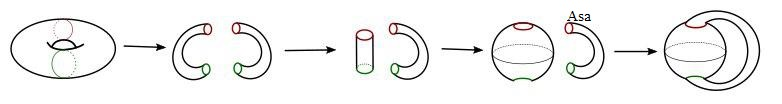
\includegraphics[scale=0.9]{asaink}
\end{figure}
Un toro es equivalente a pegar un ``asa'' a $S^2$, esto es, se hacen dos agujeros en $S^2$ y se pegan los bordes de un cilindro en ellos.
\end{flushleft}\

\begin{flushleft}\

Sea $M_2$ un toro doble

\begin{figure}[h!]
	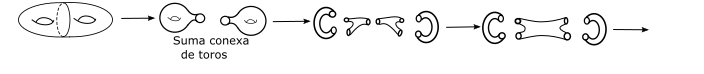
\includegraphics[scale=0.9]{asa1ink}
\end{figure}
\begin{figure}[h!]
	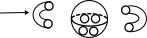
\includegraphics[scale=0.9]{asa2ink}
\end{figure}\

Así, el doble toro es el resultado de pegar dos ``asas'' a $S^2$. Consideramos ahora el triple toro $M_3$
\begin{figure}[h!]
	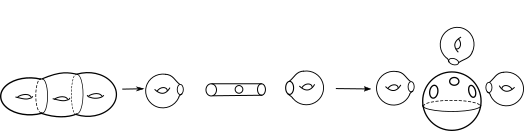
\includegraphics[scale=0.9]{asa3ink}
	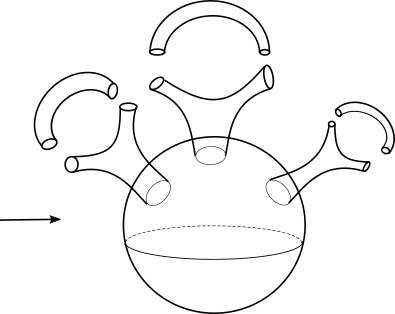
\includegraphics[scale=0.2]{asasesfera}
\end{figure}

\end{flushleft}\

Tenemos que $M_3$ se obtiene al pegar tres ``asas'' a $S^2$. En general,


\begin{teorema} La superficie de tipo I $M_n$ es el resultado de pegar $n$ ``asas'' a $S^2$.
\end{teorema}\
%\newpage
\subsubsection{Tipo II}

\begin{flushleft}
Consideremos $\Pro_2\R$
\begin{figure}[h!]
	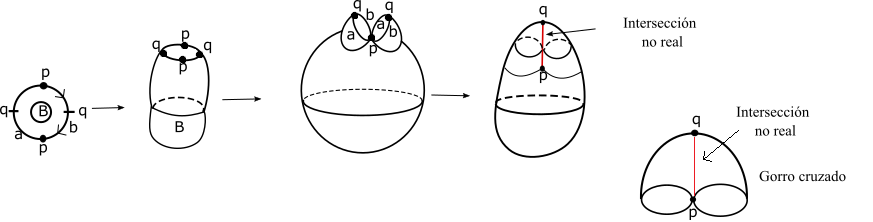
\includegraphics[scale=0.7]{gorroink}
\end{figure}
\end{flushleft}\

\begin{teorema} La superficie $N_k$ de tipo II es resultado de pegar $k$ gorros cruzados a $S^2$.
\end{teorema}

\begin{observacion}
Un gorro cruzado no es más que la banda de Möbius $\Pro_2\R\setminus B$ con la circunferencia del borde colocada en un plano. Así pues, la intersección aparente del gorro cruzado desaparece si retorcemos el borde del disco $B$, pero entonces no podemos pegar $B$ a ese borde retorcido y, a la vez,  quedarnos en el espacio tridimensional $\R^3$ sin introducir una intersección aparente. 

Debido a la imposibilidad de sumergir $\Pro_2\R$ en $\R^3$, cualquier representación tridimensional de $\Pro_2\R$ debe contener puntos dobles. Lo mismo ocurre para el resto de superficies de tipo II. Por ejemplo, si queremos representar la botella de Klein en $\R^3$
%

\definecolor{qqffqq}{rgb}{0.5,0.27,0.039}
\begin{tikzpicture}[line cap=round,line join=round,>=triangle 45,x=1.0cm,y=1.0cm]
\clip(-3,-1) rectangle (13.91820227789554,3);
%\fill[color=qqffqq,opacity=0.1](0.,0.)-- (0.,2.)--(3,2)--(3,0)--cycle;
%\fill[color=qqffqq,opacity=0.1](4.5133333333333345,0.)--(4.526666666666667,2.0133333333333336)--(6,2.0133333333333336)--(6,0.)--cycle;
\draw (0.,0.)-- (0.,2.);
\draw (0.,0.)-- (3.,0.);
\draw (0.,2.)-- (3.,2.);
\draw (3.,2.)-- (3.,0.);
\draw (4.5133333333333345,0.)-- (4.526666666666667,2.0133333333333336);
\draw (6.,2.)-- (6.,0.);
%\draw [fill=qqffqq,rotate around={-0.5184996872906775:(5.25582145324874,2.006734647481912)}] (5.25582145324874,2.006734647481912) ellipse (0.7435959297254281cm and 0.2925120722751479cm);
%\draw [fill=qqffqq,rotate around={0.:(5.26,0.)}] (5.26,0.) ellipse (0.7421639232965298cm and 0.2973336325458959cm);
\draw [rotate around={0.:(5.26,0.)}] (5.26,0.) ellipse (0.7421639232965298cm and 0.2973336325458959cm);
\draw [rotate around={-0.5184996872906775:(5.25582145324874,2.006734647481912)}] (5.25582145324874,2.006734647481912) ellipse (0.7435959297254281cm and 0.2925120722751479cm);

\draw [rotate around={-0.37943670141895985:(5.259648105152354,0.6421248326900136)},dash pattern=on 3pt off 3pt] (5.259648105152354,0.6421248326900136) ellipse (0.7438047375550998cm and 0.2291376734308262cm);
\draw [rotate around={-0.3794367014189577:(5.261976395646863,1.3220673977502335)},dash pattern=on 3pt off 3pt] (5.261976395646863,1.3220673977502335) ellipse (0.737887681672347cm and 0.21675457210560967cm);


\draw [->] (0.,2.) -- (1.5638000269466572,2.);
\draw [->] (0.,2.) -- (0.,0.9);
\draw [->] (3.,2.) -- (3.,0.9);
\draw [->] (3.,0.) -- (1.4918246161084876,0.);
\draw [->] (4.5133333333333345,2) -- (4.519545661146498,0.9);
\draw [->] (5.184841512192099,1.7160912192838051) -- (5.283414600733433,1.714202865552005);
\draw [->] (5.2772398660340025,-0.297253401817821) -- (5.1784738825715495,-0.29553424797435046);

\draw (-0.6,2.261736768042441) node[anchor=north west] {$P$};
\draw (-0.6,0.21643551005769177) node[anchor=north west] {$P$};
\draw (3.150680816505382,2.222150292081446) node[anchor=north west] {$P$};
\draw (4,2.1957593081074496) node[anchor=north west] {$P$};
\draw (4,0.2032400180706934) node[anchor=north west] {$P$};

\draw (-0.6,1.2060974090825707) node[anchor=north west] {$a$};
\draw (3.203462784453373,1.2588793770305642) node[anchor=north west] {$a$};
\draw (1.4220713662086775,2.4068871798994236) node[anchor=north west] {$b$};
\draw (1.5144398101176617,0.018503130252715997) node[anchor=north west] {$b$};
\draw (4.127147223543215,1.1665109331215755) node[anchor=north west] {$a$};
\draw (5.2,1.5) node[anchor=north west] {$S$};
\draw (5.169591090516037,2.156172832146454) node[anchor=north west] {$b$};
\draw (5.1563955985290395,-0.3) node[anchor=north west] {$b$};
\draw (5.275155026412019,0.12406706614870307) node[anchor=north west] {$F$};

\draw (3.1770718004793777,0.28241296999268367) node[anchor=north west] {$P$};

\begin{scriptsize}
\draw [fill=black] (0.,0.) circle (2.5pt);
\draw [fill=black] (0.,2.) circle (2.5pt);
\draw [fill=black] (3.,0.) circle (2.5pt);
\draw [fill=black] (3.,2.) circle (2.5pt);
\draw [fill=black] (4.5133333333333345,0.) circle (2.5pt);
\draw [fill=black] (4.526666666666667,2.0133333333333336) circle (2.5pt);
\end{scriptsize}
\end{tikzpicture}

%\begin{figure}[h!]
%	\includegraphics[scale=0.6]{FIG124.PIC}
%\end{figure}
\begin{figure}[h!]
	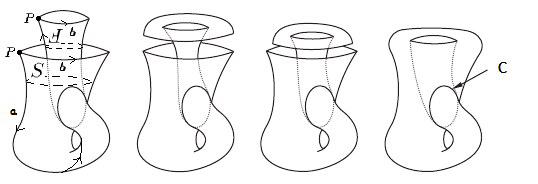
\includegraphics[scale=0.8]{kleinbottle}
\end{figure}

$C$ es la intersección aparente necesaria para tener este modelo de la botella de Klein en $\R^3$.

\end{observacion}

\end{document}